\chapter{Resultados e interpretación}
\label{cap:resultados}

Como se describiera en el \cref{cap:estrategia} en el que se presentó la
estrategia general para la búsqueda de nueva física realizada en esta Tesis, a
fin de obtener los resultados finales es necesario realizar un complejo análisis
estadístico. Los detalles de este análisis se describen en la
\cref{sec:analisis}. Este se lleva a cabo utilizando las regiones de control
para la normalización de los fondos, las regiones de validación y las regiones
donde se espera la señal de nueva física, definidas en los capítulos anteriores.
También deben ser incluidas las incertezas sistemáticas, tanto teóricas como
experimentales, las cuales se presentan en la \cref{sec:sistematicos}.

Los resultados del ajuste del likelihood se presentan en la
\cref{sec:bkgonlyfit} para las distintas regiones, para luego, de acuerdo a los
resultados obtenidos, establecer los límites a los procesos de nueva física en
la \cref{sec:model_independent}. Estos resultados son finalmente interpretados
en el contexto de un modelo particular de Supersimetría, el cual motiva el
trabajo de esta Tesis, en la \cref{sec:susy_limits}.

Por último, en la \cref{sec:13tev}, se muestran los primeros ... de 13 TeV ...


\section{Análisis Estadístico}
\label{sec:analisis}

A partir de la función likelihood general (\cref{eq:model}), se define la
función likelihood utilizada en el análisis específico de esta Tesis como:

\begin{equation}
  L(\bm{n}|\mu_s, \bm{\mu}_p, \bm{s}, \bm{b}, \bm{\alpha}) = \mathcal{P}_\text{SR} \, \times \, \mathcal{P}_\text{CRQ} \, \times \, \mathcal{P}_\text{CRW} \, \times \, \mathcal{P}_\text{CRT} \, \times \, \mathcal{C}_\text{syst}
  \label{eq:likelihood}
\end{equation}
%
donde $\bm{n}$ es el número de eventos observado en cada región (de control y
señal), y $\mu_s$ es la intensidad de la señal y constituye el parámetro de
interés del análisis. Los demás parámetros son parámetros \emph{nuisance}. Por
un lado los parámetros de normalización de los fondos ($\bm{\mu}_p$), en este
caso $\mu_Q$ para el fondo de {\gjet}, $\mu_W$ para {\wgam} y $\mu_T$ para
{\ttgam}. El número de eventos esperado de señal y fondo en cada región está
dado por $\bm{s}$ y $\bm{b}$ respectivamente, y provienen de las muestras MC o
de aquellos calculados a partir de los datos como se describe en el
\cref{cap:fondos}. Los parámetros $\alpha$ parametrizan las incertezas
sistemáticas en la señal y el fondo utilizando una distribución Gausiana.

Con la función likelihood, se construye el estadístico de prueba como el
\emph{profile likelihood ratio},

\begin{equation}
  q_{\mu_s} = -2 \ln \left( \frac{L(\mu_s,
    \doublehat{\btheta})}{L(\hat{\mu_s},\hat{\btheta})} \right)
\end{equation}
%
que será utilizado en este análisis para poner a prueba la compatibilidad de los
datos observados con las predicciones del SM.

Realizando un ajuste simultáneo a los datos en las CR (o en las CR y SR), los
parámetros descriptos anteriormente pueden ser estimados teniendo en cuenta
apropiadamente sus correlaciones e incertezas. Además, como los parámetros de
normalización de los fondos ($\bm{\mu}_p$) dependen esencialmente de las
regiones de control con una alta estadística de datos (respecto a la SR), se
reduce el impacto de estas incertezas estadísticas en las SR.

El análisis estadístico se implementó utilizando
\textsc{HistFitter}\cite{HistFitter}, una herramienta desarrollada por el grupo
de SUSY de ATLAS, que es básicamente una interfaz de \textsc{RooFit},
\textsc{RooStats}\cite{Moneta:2010pm} y
\textsc{HistFactory}\cite{Cranmer:1456844}. Además, el hecho de utilizar una
misma herramienta en distintos análisis dentro de la colaboración, permite que
su combinación estadística sea mas sencilla.


%--------------
% Sistematicos
%--------------
%\chapter{Determinación de las incertezas sistemáticas}
\section{Determinación de las incertezas sistemáticas}
\label{cap:sistematicos}

Las incertezas sistemáticas están asociadas a las predicciones de todas las
componentes del fondo y a los valores esperados de señal. Estas incertezas
pueden ser clasificadas en dos tipos: incertezas experimentales e incertezas
teóricas. Estas incertezas pueden tener impacto en el número de eventos esperado
en las CR y SR como también en los parámetros $\mu_p$ utilizados en la
extrapolación del fondo esperado.

En este Capítulo se presentan las incertezas sistemáticas consideradas y su
determinación. En la determinación de los resultados finales utilizando el
ajuste con el PLR, las predicciones de los fondos se permiten variar dentro del
tamaño de las incertezas sistemáticas y por lo tanto son restringidas por los
datos.



\subsection{Incertezas Experimentales}\label{sec:expsyst}

En esta sección se describe los procedimientos realizados para evaluar
las incertezas experimentales comunes para todos los procesos.
%% Para esto
%% se utilizó la herramienta oficial de ATLAS. %% (\textsc{SUSYTools}). %%\footnote{\texttt{SUSYTools v00-03-24-02}}.

Las incertezas sistemáticas de las estimaciones de los fondos de electrones
($\alpha_{e\to\gamma}$) y jets ($\alpha_{j\to\gamma}$) mal identificados a partir
de los datos ya se discutieron en \cref{sec:efakes,sec:jfakes}. La incerteza del
trigger tambien se discutió en \cref{sec:trigger} ($\alpha_\text{TRIG}$).

\subsubsection{Incerteza en la luminosidad}

La incerteza en la luminosidad integrada es de $\pm$2.8\% \cite{lumi2012}.
Esta es derivada siguiendo la misma metodología que la que se detalla en \cite{lumi2011},
a partir de la calibración preliminar  de la escala de luminosidad derivada
de los scans de separación de haz realizados durante Noviembre de 2012.


\subsubsection{Incerteza debida al pile-up ($\alpha_\mathrm{PRW}$)}

Como se explicó en la \cref{sec:prw} es necesario realizar
un repesado evento a evento en las muestras simuladas para modelar las condiciones
de pile-up de los datos. Para calcular la incerteza asociada a estre procedimiento
se varian los factores de escala dentro de su incerteza.

%% Siguiendo las recomendaciones de ATLAS, se utiliza
%% un factor de $1.09 \pm 0.04$ aplicado al valor medio del número de
%% interacciones por cruce de haz ($\avg{\mu}$) en el repesado debido al pile-up en las muestras simuladas
%% para describir mejor la multiplicidad de vértices del minimum bias en los datos.
%% La incerteza asociada es calculada variando este factor de escala dentro
%% de su incerteza.





%% \subsection{Incerteza en la eficiencia del trigger}

%% La eficiencia del trigger de fotones utilizado {\trigchain} es de $100^{+0}_{-1.41}$ (stat) ${}^{+0}_{-0.7}$(syst) \%,
%% relativo a candidatos a fotones aislados con $\pt > 125 \gev$ y satisfaciendo los requerimientos
%% de la selección de la región de señal descripta en la \cref{sec:event_selection}.
%% Esta fue calculada utilizando el método de \emph{bootstrap} siguiendo la descripción en \cite{Damazio:1609629}
%% y se muestra en la {\fig} \ref{fig:trigger_perf} como función del {\pt} del fotón.

%% Mas allá de la poca estadística, es claro que la eficiencia llega a un plateau antes del threshold
%% en el pt que se utiliza en este análisis. La incerteza total tiene en cuenta la limitada estadística de
%% la muestra de referencia y correciones debido a la pureza también son aplicadas.

%% \begin{figure*}[ht!]
%%   \centering
%%   \includegraphics[width=0.49\textwidth]{figures/figura}
%%   \caption{Eficiencia del trigger para {\trigchain} como funcion del {\pt} del fotón,
%%     medida a partir de los datos.}
%%   \label{fig:trigger_perf}
%% \end{figure*}



\subsubsection{Incerteza en la identificación, escala de energía y resolución de fotones y leptones}

Como se menciona en \cref{sec:fotones}, es necesario aplicar factores de escala a los fotones en las
muestras MC para corregir su eficiencia. La incerteza en estos factores es propagada
a través del análisis, siguiendo \cite{PhoEffTwiki}. %to obtain the number of tight identified photons and related variables.

La incerteza en la escala de energia de los fotones y electrones se tiene en cuenta de acuerdo a cuatro componentes\cite{EGScaleTwiki}:

\begin{itemize}\itemsep0.2cm\parskip0.2cm
\item $\alpha_\text{EGZEE}$: incerteza debido a la diferencia en la escala del $Z$
\item $\alpha_\text{EGMAT}$: incerteza debida al material
\item $\alpha_\text{EGPS}$: presampler
\item $\alpha_\text{EGLOW}$: incerteza para electrones de bajo {\pt}.
\end{itemize}


Los factores de escala están basadas en la combinación de varias medidas data-driven.
%% Los valores centrales y las incertezas son provistos por el grupo Egamma mediante la herrmaienta
%% \texttt{PhotonEfficiencyCorrectionTool}. %and propagated here to the MC background predictions ({\bf systPhId}).
%% Sin embargo, el requerimiento de aislamiento aplicado para derivar los SFs
%% (\texttt{topoEtcone40} $< 4\gev$) no es el mismo que el utilizado en este análisis. Para tener esto
%% en cuenta,

%% the tight identification efficiency was evaluated after each isolation criteria
%% for photons with $\pt>125\gev$ in both signal and \gjet\ MC. The effect is found to be very small ($<1\%$) and it is neglected.

%% Uncertainties on photon energy scale and resolution are also considered following \Ref \cite{EGScaleTwiki}.



%% \subsection{Incerteza en la identificación, escala de energía y resolución de leptones}
%%($\alpha_\text{EGZEE}$, $\alpha_\text{EGMAT}$, $\alpha_\text{EGPS}$, $\alpha_\text{EGLOW}$, $\alpha_\text{EGRES}$)}


Similar a los fotones, la incerteza en la eficiencia de identificación ($\alpha_\text{EEFF}$), y resolución de
la enegia ($\alpha_\text{EGRES}$) son consideradas siguiendo \cite{EleEffTwiki}, \cite{EGScaleTwiki}
y \cite{MCPTwiki}.





\subsubsection{Escala de energía de jets ($\alpha_\mathrm{JES}$)}

La energia de los jets es aumentada y disminuida (de forma correlacionada) en
$\pm1\sigma$ de la incerteza total de la escala de energia de jets, utilizando
una herramienta (\textsc{JetUncertainties}) provista por el grupo de Jet/Etmiss de ATLAS \cite{JesTwiki}.
Esta herramienta provee la incerteza relativa en la escala de energia de los jets,
que es la suma en cuadratura de tres componentes dependientes de: el {\pt} y $\eta$
del jet, el $\Delta R$ al jet mas cercano, y la composicion media quark-gluon de la muestra.


%% The jet energy is scaled up and down (in a fully correlated way) by the
%% $\pm1\sigma$ total uncertainty on the jet energy scale obtained using the
%% {\small \texttt{JetUncertainties}} package (v00-08-07) provided by the
%% Jet/Etmiss group \cite{JesTwiki}. The nominal analysis uses only the total JES
%% uncertainty, although it has been checked that the effect of using the reduced
%% set of JES components on the fit results is within 1\% (see
%% \cref{sec:JEScheck}).

\subsubsection{Resolucion de la energia de jets ($\alpha_\mathrm{JER}$)}

A fin de tener en cuenta una posible subestimacion de la resolucion de energia de los jets
en la simulacion MC, se realiza un smearing del {\pt} de los jets en funcion de su \pt y su $\eta$.
Cada jet es smeareado de acuerdo a una distribucion Gausiana, de media unidad y un ancho
dado por una funcion de resolucion dependiente de {\pt} y $\eta$. Para evaluar el impacto
de la incerteza sistematica debida a la resolucion de energia, el número de eventos obtenido utilizando
los jets nominales es comparado con los resultados obtenidos de los jets smeareados.
Este procedimiento tambien se realiza utilizando una herramienta provista por el grupo de Jet/Etmiss
de ATLAS.
 %% An extra \pt smearing is added to the jets based on their \pt and $\eta$ to
 %% account for a possible underestimate of the jet energy resolution in the MC
 %% simulation. This is done using the \texttt{JetResolution-02-00-03} package. The
 %% so found yield differences are then applied as a $\pm$ uncertainty.


\subsubsection{Eficiencia de identificación de {\bjets} ($\alpha_\text{BJET}$)}

La identificacion de {\bjets} solo es utilizado en la seleccion de las regiones de control CRW y CRT.
En estas regiones, se evalua la incerteza del mismo, variando los factores de escala
aplicados a cada jet en las simulaciones, que dependen de $\eta$, {\pt}, dentro del rango
que refleja la incerteza sistematica en la eficiencia medida de identificacion de {\bjets}.


%% information in this analysis. In this particular region, the b-tagging
%% uncertainty is evaluated by varying the $\eta-$, $\pt-$ and flavour-dependent
%% scale factors applied to each jet in the simulation within a range that reflects
%% the systematic uncertainty on the measured tagging efficiency and mistag rates.
%% These variations are applied separately to B-jets, C-jets and light jets,
%% leading to three uncorrelated systematic uncertainties.


\subsubsection{Término soft de \MET ($\alpha_\text{SCALEST}$, $\alpha_\text{RESOST}$)}

Al modificar la escala de enegia de los objetos o la resolucion de energia de los jets, esto
se propaga al termino correspondiente en el calculo de {\met}.

Adicionalmente, el tambien se evalua la incerteza en el termino soft de {\met}, variando
la escala de energia de los clusters, utilizando una herramienta provista por
el grupo Jet/Etmiss de ATLAS. %% (\textsc{MissingETUtility}).
Tambien se tiene en cuenta la incerteza de la resolucion en el termino soft.

%% The impact of the scales uncertainties on the soft term which enters in \MET\ is
%% estimated by varying these scales up and down using the
%% \texttt{MissingETUtility-01-03-03} package. The resolution uncertainty on the
%% cell out term is also included.




\subsection{Incertezas Teóricas}\label{sec:theosyst}


\subsubsection{Señal}\label{sec:syst_signal}

La sección eficaz para la producción de pares de gluinos  fue calculada utilizando
el programa {\nllfast} de acuerdo a las recomendaciones explicadas en \cref{sec:xs_calc}.

%% For the case of CTEQ6.6, three types of uncertainties, namely the PDF uncertainty, the scale un-
%% certainty and the αs uncertainty are taken into account. The PDF uncertainty is the 68% C.L. ranges
%% estimated with the error PDF sets for each PDF, where in case of CTEQ6.6 (MSTW2008 NLO) the varia-
%% tions of 22 (20) parameters spanning to the range of experimental uncertainties gives 44 (40) different
%% outcomes of cross sections. The αs uncertainty is defined as one half of the difference between the two
%% extreme variations in CTEQ6.6AS PDF sets.
%% The scale uncertainty is the deviations in the cross section central value by varying the factorisation
%% and the renormalisation scales by factors of two or one half. Three components are considered to be
%% independent and summed in quadrature. The same procedure is applied in case of the MSTW2008 NLO
%% except for the αs uncertainty, which is absent for MSTW2008 NLO. The nominal value is taken to be the
%% midpoint of the upper and lower envelopes. The uncertainty is assigned as the half of the full width of
%% the envelop. From definition, the uncertainty is symmetric in plus and minus sides.

%% For the $\gluino\gluino$ grid the squarks and all other SUSY partner masses are effectively set to
%% a very large scale (2.5 \TeV), so to suppress their production. Defining this large scale is arbitrary and in some cases it may
%% have a non-negligible impact in the production of the SUSY particles residing at the TeV scale (e.g. squarks at
%% high scales can still contribute to the gluino pair production process via a t-channel exchange). Thus, instead of
%% setting an explicit arbitrary value for the mass of the decoupled particle, the NLO+NLL calculation implemented
%% in {\sc NLL-Fast} assumes that this production does not interfere in any possible way with the production processes of
%% the rest of the particles.
%Thus, the particle is completely decoupled from the rest of the phenomenology at the TeV
%scale.

Los valores centrales y sus incertezas para la grid de señal están resumidos en
la \cref{tab:signal_xs_theo_unc}. Las incertezas totales van de 22.5\% para 800
{\GeV} hasta 36.8\% para 1.3 \tev.

\begin{sidewaystable}[!htbp]
  \centering
  \caption{La sección eficaz total NLO+NLL con sus incertezas y factores $k$ para los puntos de se\~nal.}
  \label{tab:signal_xs_theo_unc}

  \begin{tabular}{l|rrrrrrrrrrr}
    \hline
    $M_3$ [\gev]                     & 800                & 850               & 900                & 950               & 1000             & 1050             & 1100             & 1150             & 1200             & 1250        & 1300 \\
    $m_{\tilde{g}}$ [\gev]           & 885              & 932             & 978              & 1023            & 1068           & 1113           & 1157           & 1202           & 1246           & 1290      & 1333 \\
    \hline
    Sección eficaz (Mejor) [pb]      & 0.0690             & 0.0449            & 0.0297             & 0.01984           & 0.01341          & 0.00910          & 0.00628          & 0.00432          & 0.00301          & 0.00210     & 0.00149 \\
    Incerteza     [$\%$]             & 22.5               & 23.8              & 25.2               & 26.5         & 27.7             & 29.0             & 30.4             & 32.0             & 33.7             & 35.2        & 36.8 \\[5pt]
    PDF enc. {\cteq} [$\%$]             & \unc{22.5}{15.3}    & \unc{23.5}{15.9}   & \unc{24.6}{16.5}    & \unc{25.8}{17.1}   & \unc{26.9}{17.7}  & \unc{28.2}{18.4}  & \unc{29.4}{19.0}  & \unc{30.7}{19.7}  & \unc{32.0}{20.4}  & \unc{33.4}{21.1}    & \unc{34.8}{21.8} \\[5pt]
    PDF enc. {\mstw} [$\%$]             & \unc{9.5}{9.1}      & \unc{9.9}{9.4}     & \unc{10.2}{9.7}     & \unc{5.6}{5.0}     & \unc{10.9}{10.3}  & \unc{11.3}{10.6}  & \unc{11.8}{10.9}  & \unc{12.2}{11.2}  & \unc{12.6}{11.6}  & \unc{13.1}{11.9}    & \unc{13.6}{12.3} \\[5pt]
    Scale enc. {\cteq} [$\%$]           & \unc{9.8}{9.8}      & \unc{9.9}{9.9}     & \unc{9.9}{10.0}     & \unc{5.0}{5.0}     & \unc{10.2}{10.1}  & \unc{10.3}{10.2}  & \unc{10.4}{10.3}  & \unc{10.5}{10.4}  & \unc{10.5}{10.5}  & \unc{10.7}{10.6}    & \unc{10.8}{10.7} \\[5pt]
    Scale enc. {\mstw} [$\%$]           & \unc{10.3}{10.1}    & \unc{10.4}{10.2}   & \unc{10.5}{10.2}    & \unc{5.6}{5.3}     & \unc{10.7}{10.4}  & \unc{10.8}{10.4}  & \unc{10.9}{10.5}  & \unc{11.0}{10.6}  & \unc{11.2}{10.7}  & \unc{11.3}{10.8}    & \unc{11.4}{11.0} \\[5pt]
    $\alpha_{s}$ enc. {\cteq} [$\%$]    & \unc{6.9}{4.7}      & \unc{7.0}{4.8}     & \unc{7.2}{4.9}      & \unc{7.4}{5.0}     & \unc{7.5}{5.1}    & \unc{7.7}{5.2}    & \unc{7.9}{5.4}    & \unc{8.1}{5.5}    & \unc{8.3}{5.6}    & \unc{8.5}{5.7}      & \unc{8.7}{5.8} \\[5pt]
    $\alpha_{s}$ enc. {\mstw} [$\%$]    & \unc{3.2}{3.1}      & \unc{3.3}{3.1}     & \unc{3.3}{3.1}      & \unc{3.4}{3.1}     & \unc{3.4}{3.1}    & \unc{3.5}{3.0}    & \unc{3.5}{3.0}    & \unc{3.6}{3.0}    & \unc{3.6}{3.0}    & \unc{3.6}{2.9}      & \unc{3.7}{2.9} \\[5pt]
    Sección eficaz NLL (\cteq) [pb]  & 0.0674             & 0.044             & 0.0292             & 0.0195            & 0.0132           & 0.00896          & 0.0062           & 0.00428          & 0.00299          & 0.00209     & 0.00148 \\
    Sección eficaz NLO (\cteq) [pb]  & 0.0618             & 0.0402            & 0.0265             & 0.0177            & 0.0119           & 0.00811          & 0.00559          & 0.00384          & 0.00266          & 0.00186     & 0.00131 \\
    Sección eficaz LO  (\cteq) [pb]  & 0.0289             & 0.0186            & 0.0121             & 0.00801           & 0.00534          & 0.00358          & 0.00244          & 0.00165          & 0.00113          & 0.000776   & 0.000539 \\
    Factor $k$ (Best CS/LO)          & 2.4                & 2.41              & 2.46               & 2.48              & 2.51             & 2.54             & 2.57             & 2.62             & 2.67             & 2.71      & 2.76 \\
    \hline
  \end{tabular}

\end{sidewaystable}


\subsubsection{Producción de \ttgam}\label{sec:syst_ttbargamma}

La incerteza teórica asociada a la elección de la configuracion
utilizada en la simulación MC es
tenida en cuenta considerando variaciones en la generación de eventos
con respecto a la configuración nominal. Las variaciones consideradas
incluyen las escalas de factorización y renormalización ($0.5\times, 2\times$),
$\alpha_{s}$ y el modelo ISR/FSR (ver \cref{tab:mc_ttbar_samples}).

%are summarized below:
%
%\begin{description}
%\item {\bf Factorization and Renormalization scales}    ...
%\item $\mathbf{\alpha_s}$   ...
%\item {\bf ISR/FSR} ...
%\end{description}

La \cref{tab:syst_ttbargam_truth} resume los cambios relativos en el
número de eventos esperado en cada región de señal para cada una de las
variaciones con respecto a la muestra nominal a nivel generador.

La incerteza de cada una de las tres variaciones es simetrizada, a la mayor
entre los valores por encima y debajo, y luego sumadas en cuadratura
a la incerteza debida a la sección eficaz para obtener la incerteza teórica
total. %%o get the total theoretical uncertainty (denoted as {\bf theoSysTopG} in the fit).

\begin{table}[ht!]
  \centering
  \caption{Resumen de las incertezas teoricas del {\ttgam} obtenidas en cada región de señal.
    Todos los números están en porcentaje.}
  \label{tab:syst_ttbargam_truth}

  \begin{tabular}{l|cc}
    \hline
    & {\SRL} & {\SRH} \\
    \hline
    Escala de factorización/renormalización &  56  & 20 \\
    ISR/FSR                              &  4   & 20 \\
    $\alpha_{s}$                         &  4   &  0 \\
    %      total cross section                  &  20  &   20 \\
    \hline
    Total				&   56    &   28 \\
    \hline
  \end{tabular}

\end{table}

La diferencia principal entre todas las variaciones y la configuración nominal
aparece mayormente en los cortes en {\HT} y {\rt}. Además del efecto estadístico
obvio, es algo esperado ya que las propiedades de la actividad hadrónica del
evento son las mas sensitivas a las variaciones de escala.



\subsubsection{Producción de {\wgam} ($\alpha_{\tgam}$)}\label{sec:syst_wgamma}

Similar a lo que se realizo para estimar las incertezas teóricas del {\ttgam}, las incertezas
en el número estimado de eventos de {\wgam} fue determinada realizando el análisis a nivel
partícula para las muestras con variaciones descriptas en \cref{tab:bkg_wzgamma_samples}.
Además de las incertezas provenientes del ajuste simultaneo descripta en \cref{sec:fitconfig},
las siguientes incertezas en la aceptancia de la selección fueron consideradas:

\begin{description}
\item[Escala de factorización y renormalización] La incerteza corresponde
  a la diferencia relativa entre el número esperado de eventos predicho
  para la SR con las muestras {\sherpa} en las cuales se vario la escala
  de factorización y renormalización de forma independiente por $2\times$
  y $0.5\times$ de la escala nominal.

\item[Matching scale] The nominal matching scale between the ME and PS is 20 GeV. Alternative samples
  were generated with this scale changed to 15 and 30 \gev. The corresponding
  relative variation of yields in SR is considered as a systematic uncertainty.
\end{description}

Los valores obtenidos están resumidos en la \cref{tab:syst_wgamma_truth},
donde la incerteza total  es de  $73$\% y $39$\% para {\SRL} y
{\SRH}, respectivamente.

\begin{table}[ht!]
  \centering

  \caption{Resumen de las incertezas teóricas del {\wgam} obtenida en cada región de señal.
    Todos los números están en porcentaje.}
  \label{tab:syst_wgamma_truth}

  \begin{tabular}{l|cc}
    \hline
    & {\SRL} & {\SRH} \\
    \hline
    Escala de factorización   & $0$  & $16$ \\
    Escala de renormalización & $71$ & $33$ \\
    Escala de CKKW matching scale   & $14$ & $12$ \\
    \hline
    Total  &   $73$    &  $39$     \\
    \hline
  \end{tabular}
\end{table}



\subsubsection{Producción de fotones directos}

La normalización del fondo de {\gjet} es tomado del ajuste a datos en la CR
como se describe en \cref{bkg_gjet}. Una incerteza adicional es agregada comparando el
número de eventos en las distintas regiones de señal entre la muestra nominal
(\sherpa) y los obtenidos con otra muestra generada con {\pythia}.
Esto se realizo a nivel generador para no contar nuevamente los efectos del
detector, y se incluyo en el ajuste como $\alpha_{\gamma j}$.


\subsubsection{Otros fondos MC}

La mayor contribucion de procesos de fondo de MC en las regiones de senial viene
del {\zgam}, para el cual se utilizo una incerteza conservativa del 100\%.


%% \section{Resumen de las incertezas sistemáticas}\label{sec:syst_break}
%% \hl{Agregar tabla resumiendo todas las incertezas sistemáticas}


%% \begin{tabular}{cc}

%%   \hline
%%   \multicolumn{2}{c}{Incertezas experimentales} \\
%%   pile-up   & \\
%%   lumi      & \\
%%   trigger   & \\
%%   foton     & \\
%%   leptones  & \\
%%   jets      & \\
%%   met       & \\
%%   b-tagging & \\

%%   \hline
%%   \multicolumn{2}{c}{Incertezas teoricas} \\
%%   senal     & \\
%%   ttgam     & \\
%%   wgam      & \\
%%   phjet     & \\
%%   others    & \\
%%   \hline
%% \end{tabular}



%--------------
% Bkg-only fit
%--------------
\section{Ajuste simultáneo en las regiones de control}
\label{sec:bkgonlyfit}

Para validar los métodos utilizados para estimar los fondos, se realiza un
ajuste simultáneo utilizando únicamente las CR. El objetivo de este ajuste es
estimar el fondo total esperado en las VR y las SR, sin hacer ninguna suposición
del modelo de señal. Solo las muestras de fondo son utilizadas en el modelo, y
las CR se suponen libres de contaminación de señal. Cabe destacarse que el
ajuste se realiza solamente en las CR, y los procesos de fondo dominantes son
normalizados al número de eventos observado en cada una de las regiones. La
función likelihood utilizada es la de la \cref{eq:likelihood} sin el término de
la SR. Como los parámetros de la pdf correspondientes al fondo son compartidos
entre las diferentes regiones, el resultado del ajuste puede ser utilizado
luego, para predecir el número de eventos en las VR y SR.

Las predicciones a partir del ajuste en las CR son independientes del número de
eventos observado en cada SR y VR, lo que permite una comparación no sesgada
entre el número de eventos predicho y observado en cada región. Los resultados
de este ajuste extrapolados a las SR, también son importantes para que grupos
externos al experimento puedan hacer una prueba de hipótesis en un modelo de
nueva física, no considerado por ninguno de los experimentos del LHC.

En las siguientes secciones se muestran los resultados obtenidos
en las distintas regiones del análisis.


% Control Regions
\subsection{Resultados en las regiones de control}

El número de eventos predicho para cada proceso de fondo antes y después del ajuste en
las regiones de control puede verse en \cref{tab:fit_result_crl,tab:fit_result_crh},
comparado con el número de eventos observado.
Estas regiones no solo determinan la normalización de los proceso de fondo dominante
en cada una, sino que también restringen las incertezas sistemáticas aplicadas todos
los fondos.

En la \cref{tab:bkgonly_mus} se presentan los parámetros de normalización de
los fondos {\wgam} ($\mu_W$), {\ttgam} ($\mu_T$) y {\gjet}
($\mu_Q$), obtenidos del ajuste realizado en las regiones de control.
En su mayoría, los factores resultan consistentes con la unidad dentro de sus incertezas.

En la \cref{fig:fit_unc_nuisance} se encuentran resumidos todos los parámetros
del ajuste simultáneo (las incertezas sistemáticas y los factores de
normalización de los fondos). Los valores de los puntos representan los
\emph{pulls} en los parámetros \emph{nuisance}, lo que indica el apartamiento de los valores
centrales luego del ajuste. Las líneas de error representan el
 grado de disminución de las incertezas por el
ajuste. Si este es muy grande puede resultar en un aumento artificial
en la sensibilidad a nueva física, reduciendo las incertezas sistemáticas.
Por este motivo resulta importante
chequear el comportamiento de los parámetros \emph{nuisance} después del ajuste.
En este caso se observa que todos los parámetros dan resultados razonables
y el valor central es practicamente cero.

Los puntos de la derecha de la \cref{fig:fit_unc_nuisance}, después de la linea
punteada, representan los parámetros de normalización de los distintos fondos. Se
puede ver que todos los valores centrales estan contenidos dentro de una desviación estándar.
La correlación de los distintos parámetros se muestran en la \cref{fig:fit_corrmatrix}.

\begin{table}[!htb]
  \centering

  \caption{Resultados del ajuste en las CR correspondientes a {\SRL}, con una luminosidad integrada total de 20.3 \ifb.
    El número de eventos observado es comparado con el número de eventos esperado de fondo, después de la correspondiente
    normalización en las CR. En la parte inferior de la tabla se muestran también lo valores nominales del fondo antes de
    la correspondiente normalización. Las incertezas incluyen la incerteza estadística y sistemática.}
  \label{tab:fit_result_crl}

  {\small\begin{tabularx}{\textwidth}{|z{3.2mm}|z{5cm}RRR}
\hline
\multicolumn{2}{l}{\hspace{6.5mm} \bf Regiones de control}           & {\CRQL}            & {\CRWL}            & {\CRTL}              \\
\hline
\multicolumn{2}{l}{\hspace{6.5mm} Eventos observados}                             & $1348$              & $8$              & $18$                    \\
\hline
\multirow{11}{*}{\rotatebox[origin=c]{90}{Después}} & Eventos esperados SM                           & $1347.21 \pm 36.51$          & $8.00 \pm 2.75$          & $18.00 \pm 4.16$              \\
\cline{2-5}
 & {\wgam}                                 & $0.28 \pm 0.27$          & $5.24 \pm 3.07$          & $3.15 \pm 1.94$              \\
 & {\ttgam}                                & $2.22 \pm 1.31$          & $1.33 \pm 0.73$          & $10.66 \pm 4.92$              \\
 & {\ttgam} (had)                          & $28.46 \pm 16.90$          & $0.00 \pm 0.00$          & $0.00 \pm 0.00$              \\
 & {\vqqgam}                               & $39.30 \pm 24.90$          & $0.00 \pm 0.00$          & $0.00 \pm 0.00$              \\
 & {\tgam}                                 & $0.24 \pm 0.04$          & $0.22 \pm 0.06$          & $1.24 \pm 0.24$              \\
 & {\zllgam}                               & $0.08_{-0.08}^{+0.10}$          & $0.14_{-0.14}^{+0.14}$          & $0.11_{-0.11}^{+0.11}$              \\
 & {\znngam}                               & $0.00 \pm 0.00$          & $0.00 \pm 0.00$          & $0.00 \pm 0.00$              \\
 & {\gjet}                                 & $1155.79 \pm 68.55$          & $0.13 \pm 0.04$          & $0.01 \pm 0.01$              \\
 & $e\rightarrow\gamma$                    & $5.34 \pm 0.89$          & $0.26 \pm 0.05$          & $1.29 \pm 0.21$              \\
 & $j\rightarrow\gamma$                    & $115.48 \pm 54.49$          & $0.69 \pm 0.32$          & $1.54 \pm 0.72$              \\
\hline
\multirow{11}{*}{\rotatebox[origin=c]{90}{Antes}} & Eventos esperados SM                            & $1397.30$          & $6.29$          & $14.14$              \\
\cline{2-5}
& {\wgam}                                & $0.21$          & $3.90$          & $2.34$              \\
& {\ttgam}                  & $1.59$          & $0.95$          & $7.61$              \\
& {\ttgam} (had)         & $20.31$          & $0.00$          & $0.00$              \\
& {\vqqgam}                   & $29.25$          & $0.00$          & $0.00$              \\
& {\tgam}                  & $0.24$          & $0.22$          & $1.24$              \\
& {\zllgam}    & $0.08$          & $0.14$          & $0.11$              \\
& {\znngam}      & $0.00$          & $0.00$          & $0.00$              \\
& {\gjet}                                & $1224.79$          & $0.14$          & $0.01$              \\
& $e\rightarrow\gamma$             & $5.34$          & $0.26$          & $1.29$              \\
& $j\rightarrow\gamma$             & $115.48$          & $0.69$          & $1.54$              \\
\hline
\end{tabularx}
}

\end{table}


\begin{table}[!htb]

  \caption{Resultados del ajuste en las CR correspondientes a {\SRH}, con una luminosidad integrada total de 20.3 \ifb.
    El número de eventos observado es comparado con el número de eventos esperado de fondo, después de la correspondiente
    normalización en las CR. En la parte inferior de la tabla se muestran también lo valores nominales del fondo antes de
    la correspondiente normalización. Las incertezas incluyen la incerteza estadística y sistemática.}
  \label{tab:fit_result_crh}

  \begin{tabularx}{\textwidth}{z{5cm}RRR}
\hline
{\bf Regiones de control}           & {\CRQH}     & {\CRWH}            & {\CRTH}              \\
\hline
Eventos observados          & $216$              & $25$              & $17$                    \\
\hline
Eventos esperados SM        & $216.03 \pm 14.53$          & $25.00 \pm 4.99$          & $17.00 \pm 4.08$              \\
\hline
{\wgam}         & $0.10 \pm 0.08$          & $19.32 \pm 5.62$          & $4.66 \pm 1.43$              \\
{\ttgam}          & $0.04 \pm 0.04$          & $1.91 \pm 1.34$          & $6.88 \pm 4.63$              \\
{\ttgam} (had)          & $0.31 \pm 0.24$          & $0.00 \pm 0.00$          & $0.00 \pm 0.00$              \\
V($\to$ qq)$+\gamma$          & $3.46 \pm 1.53$          & $0.00 \pm 0.00$          & $0.00 \pm 0.00$              \\
single-$t$ + $\gamma$          & $0.01_{-0.01}^{+0.02}$          & $0.54 \pm 0.06$          & $1.51 \pm 0.18$              \\
Z($\rightarrow\ell\ell$) + $\gamma$          & $0.00 \pm 0.00$          & $0.57 \pm 0.57$          & $0.19_{-0.19}^{+0.19}$              \\
Z($\rightarrow\nu\nu$) + $\gamma$          & $0.00 \pm 0.00$          & $0.00 \pm 0.00$          & $0.00 \pm 0.00$              \\
$\gamma$ + jet          & $193.31 \pm 16.91$          & $0.02_{-0.02}^{+0.94}$          & $0.00 \pm 0.00$              \\
$e\rightarrow\gamma$ fakes          & $0.27 \pm 0.04$          & $0.49 \pm 0.08$          & $2.31 \pm 0.37$              \\
$j\rightarrow\gamma$ fakes          & $18.52 \pm 8.70$          & $2.14 \pm 0.99$          & $1.46 \pm 0.68$              \\
\hline
Eventos esperado SM (MC/DD)              & $179.24$          & $22.94$          & $22.04$              \\
\hline
MC {\wgam}               & $0.08$          & $15.62$         & $3.76$              \\
MC {\ttgam}              & $0.08$          & $3.57$          & $12.82$              \\
MC {\ttgam} (had)        & $0.58$          & $0.00$          & $0.00$              \\
MC {\vqqgam}             & $2.80$          & $0.00$          & $0.00$              \\
MC {\tgam}               & $0.01$          & $0.54$          & $1.51$              \\
MC {\zllgam}             & $0.00$          & $0.57$          & $0.19$              \\
MC {\znngam}             & $0.00$          & $0.00$          & $0.00$              \\
MC {\gjet}               & $156.91$        & $0.02$          & $0.00$              \\
DD $e\rightarrow\gamma$  & $0.27$          & $0.49$          & $2.31$              \\
DD $j\rightarrow\gamma$  & $18.50$         & $2.14$          & $1.46$              \\
\hline
\end{tabularx}


\end{table}


\begin{table}[!htb]
  \centering

  \caption{Factores de normalización para los fondos
    {\wgam} ($\mu_{W}$), {\ttgam} ($\mu_{T}$) y {\gjet} ($\mu_{Q}$), obtenidos
    del ajuste combinado en las CR. Las incertezas mostradas son solo estadísticas.}
  \label{tab:bkgonly_mus}

  \begin{tabular}{lccc}
    \hline
    &       $\mu_{Q}$ &       $\mu_{W}$ &       $\mu_{T}$ \\
    \hline
    \SRL & $0.94 \pm 0.44$ & $1.34 \pm 0.89$ & $1.40 \pm 0.77$ \\
    \SRH & $1.22 \pm 0.58$ & $1.24 \pm 0.39$ & $0.54 \pm 0.37$ \\
    \hline
  \end{tabular}

\end{table}


\begin{figure}[!htb]
  \centering

  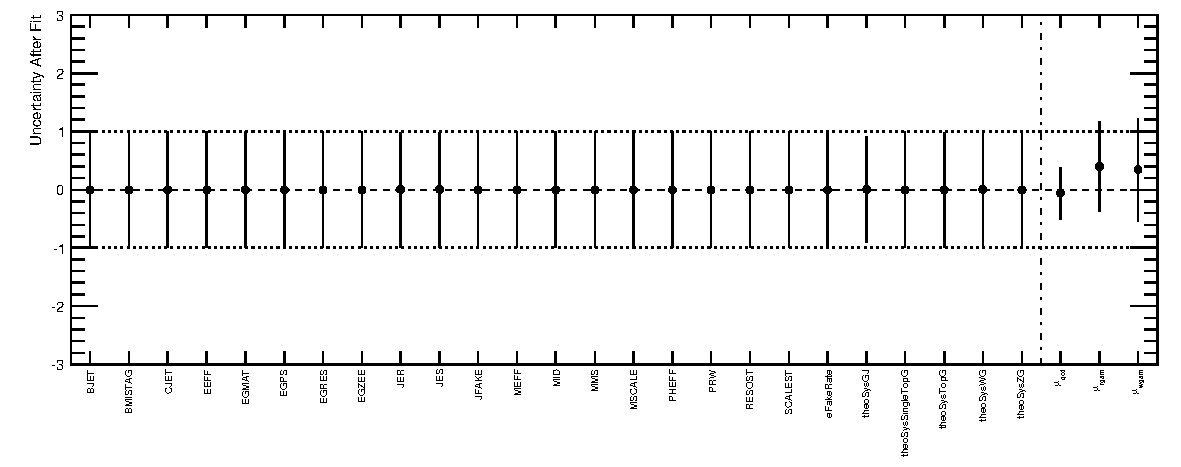
\includegraphics[width=0.8\textwidth]{syst_pull_afterFit_srl} \\
  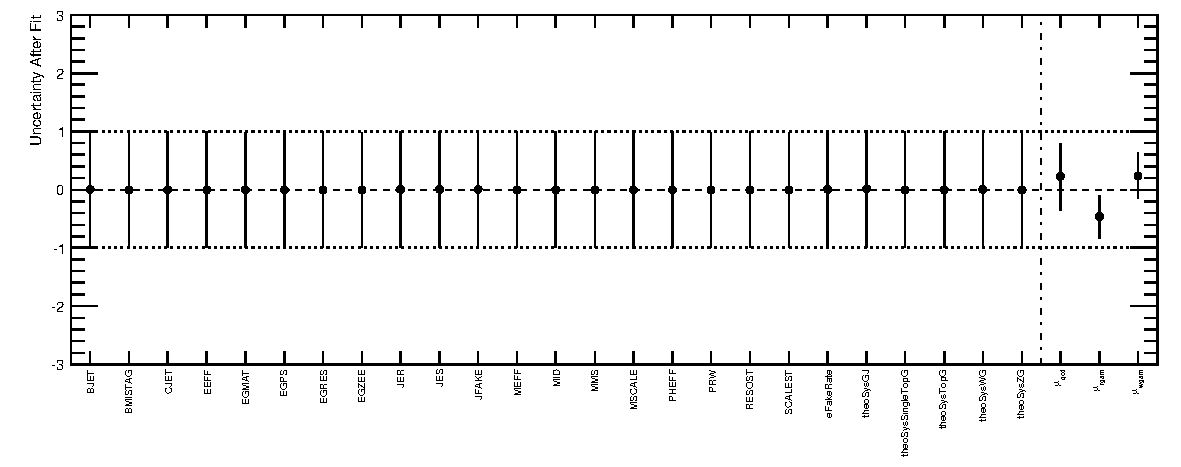
\includegraphics[width=0.8\textwidth]{syst_pull_afterFit_srh}

  \caption{Resumen de los parámetros después del ajuste para {\SRL} (arriba) y {\SRH} (abajo).}
  \label{fig:fit_unc_nuisance}

\end{figure}


\begin{figure}[!htb]
  \centering

  \includegraphics[width=0.49\textwidth]{corr_matrix_srl}
  \includegraphics[width=0.49\textwidth]{corr_matrix_srh}

  \caption{Matriz de correlación de los parámetros del ajuste, correspondientes a {\SRL} (izquierda) y {\SRH} (derecha).}
  \label{fig:fit_corrmatrix}

\end{figure}


%% \begin{figure}[!htbp]
%%   \centering

%%   \includegraphics[width=0.49\textwidth]{can_crql_met_et_afterFit}
%%   \includegraphics[width=0.49\textwidth]{can_crql_rt4_afterFit} \\

%%   \includegraphics[width=0.49\textwidth]{can_crwl_met_et_afterFit}
%%   \includegraphics[width=0.49\textwidth]{can_crwl_rt4_afterFit} \\

%%   \includegraphics[width=0.49\textwidth]{can_crtl_met_et_afterFit}
%%   \includegraphics[width=0.49\textwidth]{can_crtl_rt4_afterFit} \\

%%    \caption{Distribuciones observadas de {\met} (izquierda) y {\rt} (derecha) en las
%%      regiones de control {\CRQL} (arriba), {\CRWL} (medio) y {\CRTL} (abajo),
%%      después del ajuste combinado.}
%%    \label{fig:bkgfit_crl_after}

%% \end{figure}


%% \begin{figure}[!htbp]
%%   \centering

%%   \includegraphics[width=0.49\textwidth]{can_crqh_met_et_afterFit}
%%   \includegraphics[width=0.49\textwidth]{can_crqh_rt4_afterFit} \\

%%   \includegraphics[width=0.49\textwidth]{can_crwh_met_et_afterFit}
%%   \includegraphics[width=0.49\textwidth]{can_crwh_rt4_afterFit} \\

%%   \includegraphics[width=0.49\textwidth]{can_crth_met_et_afterFit}
%%   \includegraphics[width=0.49\textwidth]{can_crth_rt4_afterFit} \\

%%   \caption{Distribuciones observadas de {\met} (izquierda) y {\HT} (derecha) en las
%%     regiones de control {\CRQH} (arriba), {\CRWH} (medio) y {\CRTH} (abajo),
%%     después del ajuste combinado.}
%%   \label{fig:bkgfit_crh_after}

%% \end{figure}





%% Validation Regions
\subsection{Resultados en las regiones de validación}

Los factores de normalización calculados a partir del ajuste simultáneo en las
CR, y detallados en la \cref{tab:bkgonly_mus}, son utilizados para estimar los fondos
en las VR, donde se compara el fondo esperado con los datos observados, a fin de
validar la extrapolación que luego se hará a la SR.

En las \cref{tab:fit_result_vrl,tab:fit_result_vrh} se presentan los resultados
para las distintas regiones de validación asociadas a {\SRL} y {\SRH},
respectivamente, y en las \cref{fig:bkgfit_vr} pueden verse las distribuciones
de algunos observables en estas mismas regiones. En general, el número de
eventos de fondo predicho está en buen acuerdo con el número de eventos
observado dentro de las incertezas, lo que permite validar el método empleado y
la viabilidad de utilizar la estimación del número de eventos de fondo en las
SR, lo cual puede observarse más fácilmente en la
\cref{fig:fit_region_composition} donde se presentan los \emph{pull} para las
distintas regiones, definido como $\frac{n_\text{obs} - n_\text{exp}}{\sigma_\text{tot}}$.
Decir lo que es sigmatot.
El mismo acuerdo puede verse de las distribuciones de los
observables en las VR, las cuales muestran que no existen problemas en el
modelado de los distintos observables.

Habiendo validado el método de obtención del fondo contaminante en la región
donde se espera la señal de nueva física, se procedió a la utilización de los
datos experimentales en las denominadas regiones de señal, cuyos resultados
pueden verse en la siguiente sección.


\begin{table}[!htb]

  \caption{Resultados del ajuste en las VR correspondientes a {\SRL}.
    El número de eventos observado es comparado con el número de eventos esperado de fondo, después de la correspondiente
    normalización en las CR. Las incertezas incluyen la incerteza estadística y sistemática.}
  \label{tab:fit_result_vrl}

  \begin{tabularx}{\textwidth}{z{4cm}RRRR}
\hline
{\bf Regiones de validación}                  & VRQ            & VRM75            & VRM100            & VRR              \\
\hline
Eventos observados        & $0$            & $54$              & $7$              & $24$                    \\
\hline
Eventos esperados SM    & $0.39 \pm 0.23$  & $51.17 \pm 47.04$          & $13.24 \pm 5.51$          & $24.32 \pm 6.26$              \\
\hline
{\wgam}          & $0.04 \pm 0.04$    & $0.89 \pm 0.79$          & $0.45 \pm 0.40$          & $6.82 \pm 5.74$              \\
{\ttgam}          & $0.30 \pm 0.20$             & $2.55 \pm 1.65$          & $1.54 \pm 1.01$          & $4.74 \pm 2.80$              \\
{\ttgam}  (had)    & $0.02 \pm 0.02$         & $1.69 \pm 1.08$          & $0.38 \pm 0.25$          & $0.00 \pm 0.00$              \\
{\vqqgam}          & $0.00 \pm 0.00$              & $2.45 \pm 2.17$          & $0.82 \pm 0.82$          & $0.00 \pm 0.00$              \\
{\tgam}          & $0.01 \pm 0.01$             & $0.25 \pm 0.10$          & $0.15 \pm 0.06$          & $0.45 \pm 0.08$              \\
{\zllgam}         & $0.00 \pm 0.00$          & $0.08_{-0.08}^{+0.08}$          & $0.04_{-0.04}^{+0.04}$          & $0.08_{-0.08}^{+0.08}$              \\
{\znngam}         & $0.00 \pm 0.00$           & $0.10_{-0.10}^{+0.12}$          & $0.07_{-0.07}^{+0.07}$          & $1.71_{-1.71}^{+1.75}$              \\
{\gjet}        & $0.01_{-0.01}^{+0.07}$            & $35.97_{-35.97}^{+44.72}$          & $7.87 \pm 4.47$          & $2.37 \pm 1.17$              \\
$e\rightarrow\gamma$           & $0.01 \pm 0.00$        & $2.56 \pm 0.72$          & $1.32 \pm 0.43$          & $6.09 \pm 1.14$              \\
$j\rightarrow\gamma$           & $0.00 \pm 0.00$          & $4.63 \pm 2.41$          & $0.60 \pm 0.33$          & $2.06 \pm 0.98$              \\
\hline
%% Eventos esperados SM (MC/DD)              & $0.29$           & $51.24$          & $12.83$          & $21.36$              \\
%% \hline
%% MC W + $\gamma$          & $0.03$                & $0.66$          & $0.33$          & $5.08$              \\
%% MC $t\bar{t}$ + $\gamma$          & $0.21$         & $1.82$          & $1.10$          & $3.39$              \\
%% MC $t\bar{t}$ + $\gamma$ (had)          & $0.01$            & $1.20$          & $0.27$          & $0.00$              \\
%% MC V($\to$ qq)$+\gamma$          & $0.00$             & $1.82$          & $0.61$          & $0.00$              \\
%% MC single-$t$ + $\gamma$          & $0.01$               & $0.25$          & $0.15$          & $0.45$              \\
%% MC Z($\rightarrow\ell\ell$) + $\gamma$          & $0.00$              & $0.08$          & $0.04$          & $0.08$              \\
%% MC Z($\rightarrow\nu\nu$) + $\gamma$          & $0.00$                & $0.10$          & $0.07$          & $1.71$              \\
%% MC $\gamma$ + jet          & $0.01$              & $38.11$          & $8.34$          & $2.51$              \\
%% DD $e\rightarrow\gamma$         & $0.01$             & $2.56$          & $1.32$          & $6.09$              \\
%% DD $j\rightarrow\gamma$         & $0.00$              & $4.63$          & $0.60$          & $2.06$              \\
%% \hline
\end{tabularx}


  \bigskip

  \begin{tabularx}{\textwidth}{z{4cm}RRRR}
\hline
{\bf Regiones de validación}                   & VRWR            & VRWM            & VRTR            & VRTM              \\
\hline
Eventos observados                             & $0$             & $5$             & $1$             & $3$                    \\
\hline
Eventos esperados SM                           & $0.20 \pm 0.15$          & $3.41 \pm 1.41$          & $0.76 \pm 0.30$          & $3.52 \pm 0.84$              \\
\hline
{\wgam}               & $0.13 \pm 0.10$          & $2.39 \pm 1.47$          & $0.04 \pm 0.03$          & $1.04 \pm 0.65$              \\
{\ttgam}              & $0.04_{-0.04}^{+0.07}$   & $0.41 \pm 0.21$          & $0.46 \pm 0.28$          & $1.86 \pm 0.92$              \\
{\ttgam} (had)        & $0.00 \pm 0.00$          & $0.00 \pm 0.00$          & $0.00 \pm 0.00$          & $0.00 \pm 0.00$              \\
{\vqqgam}             & $0.00 \pm 0.00$          & $0.00 \pm 0.00$          & $0.00 \pm 0.00$          & $0.00 \pm 0.00$              \\
{\tgam}               & $0.03 \pm 0.02$          & $0.04 \pm 0.01$          & $0.08 \pm 0.03$          & $0.19 \pm 0.04$              \\
{\zllgam}             & $0.00 \pm 0.00$          & $0.06_{-0.06}^{+0.06}$   & $0.02_{-0.02}^{+0.02}$   & $0.00 \pm 0.00$              \\
{\znngam}             & $0.00 \pm 0.00$          & $0.00 \pm 0.00$          & $0.00 \pm 0.00$          & $0.00 \pm 0.00$              \\
{\gjet}               & $0.00 \pm 0.00$          & $0.00 \pm 0.00$          & $0.00 \pm 0.00$          & $0.00 \pm 0.00$              \\
$e\rightarrow\gamma$  & $0.00 \pm 0.00$          & $0.07 \pm 0.02$          & $0.08 \pm 0.02$          & $0.17 \pm 0.03$              \\
$j\rightarrow\gamma$  & $0.00 \pm 0.00$          & $0.43 \pm 0.21$          & $0.09 \pm 0.04$          & $0.26 \pm 0.12$              \\
\hline
%% MC exp. SM events              & $0.16$          & $2.68$          & $0.62$          & $2.72$              \\
%% \noalign{\smallskip}\hline\noalign{\smallskip}
%%         MC exp. W + $\gamma$ events         & $0.09$          & $1.78$          & $0.03$          & $0.77$              \\
%%         MC exp. $t\bar{t}$ + $\gamma$ events         & $0.03$          & $0.29$          & $0.33$          & $1.33$              \\
%%         MC exp. $t\bar{t}$ + $\gamma$ (had) events         & $0.00$          & $0.00$          & $0.00$          & $0.00$              \\
%%         MC exp. V($\to$ qq)$+\gamma$ events         & $0.00$          & $0.00$          & $0.00$          & $0.00$              \\
%%         MC exp. single-$t$ + $\gamma$ events         & $0.03$          & $0.04$          & $0.08$          & $0.19$              \\
%%         MC exp. Z($\rightarrow\ell\ell$) + $\gamma$ events         & $0.00$          & $0.06$          & $0.02$          & $0.00$              \\
%%         MC exp. Z($\rightarrow\nu\nu$) + $\gamma$ events         & $0.00$          & $0.00$          & $0.00$          & $0.00$              \\
%%         MC exp. $\gamma$ + jet events         & $0.00$          & $0.00$          & $0.00$          & $0.00$              \\
%%         DD exp. $e\rightarrow\gamma$ fakes events         & $0.00$          & $0.07$          & $0.08$          & $0.17$              \\
%%         DD exp. $j\rightarrow\gamma$ fakes events         & $0.00$          & $0.43$          & $0.09$          & $0.26$              \\

%% \noalign{\smallskip}\hline\noalign{\smallskip}
\end{tabularx}


\end{table}


\begin{table}[!htb]

  \caption{Resultados del ajuste en las VR correspondientes a {\SRH}.
    El número de eventos observado es comparado con el número de eventos esperado de fondo, después de la correspondiente
    normalización en las CR. Las incertezas incluyen la incerteza estadística y sistemática.}
  \label{tab:fit_result_vrh}

  \begin{tabularx}{\textwidth}{LRR}
\hline
{\bf Regiones de validación}           & VRQ                      & VRH                          \\
\hline
Eventos observados                     & $2$                      & $4$                          \\
\hline
Eventos esperados SM                   & $0.89 \pm 0.32$          & $3.39 \pm 1.69$              \\
\hline
{\wgam}                                & $0.34 \pm 0.19$          & $1.18 \pm 0.55$              \\
{\ttgam}                               & $0.07 \pm 0.05$          & $0.11 \pm 0.08$              \\
{\ttgam} (had)                         & $0.01 \pm 0.01$          & $0.00 \pm 0.00$              \\
%% {\vqqgam}                              & $0.00 \pm 0.00$          & $0.00 \pm 0.00$              \\
{\tgam}                                & $0.03 \pm 0.01$          & $0.01 \pm 0.00$              \\
{\zllgam}                              & $0.02_{-0.02}^{+0.02}$   & $0.00 \pm 0.00$              \\
{\znngam}                              & $0.08_{-0.08}^{+0.08}$   & $1.60_{-1.60}^{+1.61}$       \\
{\gjet}                                & $0.19 \pm 0.11$          & $0.00 \pm 0.00$              \\
$e\rightarrow\gamma$                   & $0.00 \pm 0.00$          & $0.15 \pm 0.03$              \\
$j\rightarrow\gamma$                   & $0.17 \pm 0.09$          & $0.34 \pm 0.16$              \\
\hline
%% MC exp. SM               & $0.86$          & $3.25$              \\
%% \hline
%% MC W + $\gamma$          & $0.27$          & $0.96$              \\
%% MC $t\bar{t}$ + $\gamma$          & $0.12$          & $0.20$              \\
%% MC $t\bar{t}$ + $\gamma$ (had)          & $0.02$          & $0.00$              \\
%% MC V($\to$ qq)$+\gamma$          & $0.00$          & $0.00$              \\
%% MC single-$t$ + $\gamma$          & $0.03$          & $0.01$              \\
%% MC Z($\rightarrow\ell\ell$) + $\gamma$          & $0.02$          & $0.00$              \\
%% MC Z($\rightarrow\nu\nu$) + $\gamma$          & $0.08$          & $1.60$              \\
%% MC $\gamma$ + jet          & $0.15$          & $0.00$              \\
%% DD $e\rightarrow\gamma$          & $0.00$          & $0.15$              \\
%% DD $j\rightarrow\gamma$          & $0.17$          & $0.34$              \\
%% \hline
\end{tabularx}


  \bigskip

  \begin{tabularx}{\textwidth}{z{4cm}RRRR}
\hline
{\bf Regiones de validación}                      & VRWH            & VRWM            & VRTH            & VRTM              \\
\hline
Eventos observados                                & $1$              & $5$              & $2$              & $2$                    \\
\hline
Eventos esperados SM                              & $1.25 \pm 0.38$          & $4.38 \pm 1.14$          & $0.83 \pm 0.26$          & $1.76 \pm 0.38$              \\
\hline
{\wgam}                      & $1.08 \pm 0.38$          & $3.75 \pm 1.17$          & $0.28 \pm 0.17$          & $1.08 \pm 0.35$              \\
{\ttgam}                     & $0.04 \pm 0.04$          & $0.13 \pm 0.09$          & $0.17 \pm 0.13$          & $0.38 \pm 0.27$              \\
%% {\ttgam} (had)               & $0.00 \pm 0.00$          & $0.00 \pm 0.00$          & $0.00 \pm 0.00$          & $0.00 \pm 0.00$              \\
%% {\vqqgam}                    & $0.00 \pm 0.00$          & $0.00 \pm 0.00$          & $0.00 \pm 0.00$          & $0.00 \pm 0.00$              \\
{\tgam}                      & $0.02 \pm 0.01$          & $0.02 \pm 0.01$          & $0.15 \pm 0.04$          & $0.08 \pm 0.02$              \\
{\zllgam}                    & $0.00 \pm 0.00$          & $0.00 \pm 0.00$          & $0.02_{-0.02}^{+0.02}$   & $0.00 \pm 0.00$              \\
%% {\znngam}                    & $0.00 \pm 0.00$          & $0.00 \pm 0.00$          & $0.00 \pm 0.00$          & $0.00 \pm 0.00$              \\
{\gjet}                      & $0.02 \pm 0.01$          & $0.00 \pm 0.00$          & $0.00 \pm 0.00$          & $0.00 \pm 0.00$              \\
$e\rightarrow\gamma$         & $0.00 \pm 0.00$          & $0.04 \pm 0.01$          & $0.05 \pm 0.01$          & $0.05 \pm 0.01$              \\
$j\rightarrow\gamma$         & $0.09 \pm 0.04$          & $0.43 \pm 0.20$          & $0.17 \pm 0.09$          & $0.17 \pm 0.08$              \\
\hline
%% %%
%% MC exp. SM events              & $1.07$          & $3.78$          & $0.92$          & $1.88$              \\
%% \noalign{\smallskip}\hline\noalign{\smallskip}
%% %%
%%         MC exp. W + $\gamma$ events         & $0.87$          & $3.04$          & $0.23$          & $0.87$              \\
%% %%
%%         MC exp. $t\bar{t}$ + $\gamma$ events         & $0.08$          & $0.25$          & $0.31$          & $0.71$              \\
%% %%
%%         MC exp. $t\bar{t}$ + $\gamma$ (had) events         & $0.00$          & $0.00$          & $0.00$          & $0.00$              \\
%% %%
%%         MC exp. V($\to$ qq)$+\gamma$ events         & $0.00$          & $0.00$          & $0.00$          & $0.00$              \\
%% %%
%%         MC exp. single-$t$ + $\gamma$ events         & $0.02$          & $0.02$          & $0.15$          & $0.08$              \\
%% %%
%%         MC exp. Z($\rightarrow\ell\ell$) + $\gamma$ events         & $0.00$          & $0.00$          & $0.02$          & $0.00$              \\
%% %%
%%         MC exp. Z($\rightarrow\nu\nu$) + $\gamma$ events         & $0.00$          & $0.00$          & $0.00$          & $0.00$              \\
%% %%
%%         MC exp. $\gamma$ + jet events         & $0.02$          & $0.00$          & $0.00$          & $0.00$              \\
%% %%
%%         DD exp. $e\rightarrow\gamma$ fakes events         & $0.00$          & $0.04$          & $0.05$          & $0.05$              \\
%% %%
%%         DD exp. $j\rightarrow\gamma$ fakes events         & $0.09$          & $0.43$          & $0.17$          & $0.17$              \\
%% %%     \\
%% \noalign{\smallskip}\hline\noalign{\smallskip}
\end{tabularx}


\end{table}


\begin{figure}[!htbp]
  \centering

  \includegraphics[width=0.49\textwidth]{can_vrm75l_met_et_afterFit}
  \includegraphics[width=0.49\textwidth]{can_vrm75l_rt4_afterFit} \\

  \includegraphics[width=0.49\textwidth]{can_vrh_met_et_afterFit}
  \includegraphics[width=0.49\textwidth]{can_vrh_ht_afterFit} \\

  \caption{Distribuciones observadas en algunas de las regiones de validación, después del ajuste combinado.}
  \label{fig:bkgfit_vr}

\end{figure}




\subsection{Resultados en las regiones de señal}

Las predicciones del fondo luego del ajuste simultáneo en las CR son presentadas
en la \cref{tab:fit_result_sr} para las regiones de señal, {\SRL} y {\SRH}, donde
se espera señal de nueva física,
conjuntamente con el número de eventos de datos observados. El acuerdo entre los
datos observados y el fondo esperado es bueno y no se observa un exceso
significativo de datos por sobre los predichos en ninguna de las SR.
El número de eventos esperado a partir de procesos del {\SM}  en la region {\SRL} y
{\SRH} es de $1.27\pm0.43$ y $0.84\pm0.38$, respectivamente, mientras que el
número de eventos observado en ambas SR es de 2.

\begin{table}[!htbp]
  \centering

  \caption{Resultados del ajuste en las SR, con una luminosidad integrada total
    de 20.3 \ifb. El número de eventos observado es comparado con el número de
    eventos esperado de fondo, después de la correspondiente normalización en
    las CR. Las incertezas incluyen la incerteza estadística y sistemática.}
  \label{tab:fit_result_sr}

  \begin{tabularx}{\textwidth}{LRR}
\hline
{\bf Regiones de señal} & {\SRL} & {\SRH}  \\
\hline
Eventos observados                         & $2$                        &  $2$                          \\
\hline
Eventos esperados SM                       & $1.27 \pm 0.43$            &  $0.84 \pm 0.38$              \\
\hline
{\wgam}                                    & $0.13 \pm 0.12$            &  $0.54 \pm 0.28$              \\
{\ttgam}                                    & $0.64 \pm 0.40$            &  $0.05 \pm 0.05$              \\
{\vqqgam}                                  & $0.00 \pm 0.00$            &  $0.00 \pm 0.00$              \\
{\tgam}                                    & $0.06 \pm 0.02$            &  $0.03 \pm 0.01$              \\
{\zllgam}                                  & $0.00 \pm 0.00$            &  $0.00 \pm 0.00$              \\
{\znngam}                                  & $0.03_{-0.03}^{+0.05}$     &  $0.21_{-0.21}^{+0.23}$       \\
{\gjet}                                    & $0.00_{-0.00}^{+0.06}$     &  $0.00 \pm 0.00$              \\
$e\to\gamma$                       & $0.38 \pm 0.10$            &  $0.00 \pm 0.00$              \\
$j\to\gamma$                       & $0.02_{-0.02}^{+0.08}$     &  $0.00_{-0.00}^{+0.08}$       \\
\hline
\end{tabularx}


\end{table}


Las distribuciones de {\met} para {\SRL} y {\SRH} se muestran en la
\cref{fig:met_sr} para datos y también para el fondo esperado después del
ajuste en las CR. Se puede ver el buen acuerdo en la zona de bajo {\met} y las
flechas indican la zona de las SR utilizadas para obtener los resultados finales
del presente análisis.

\begin{figure}[!htbp]

  \centering

  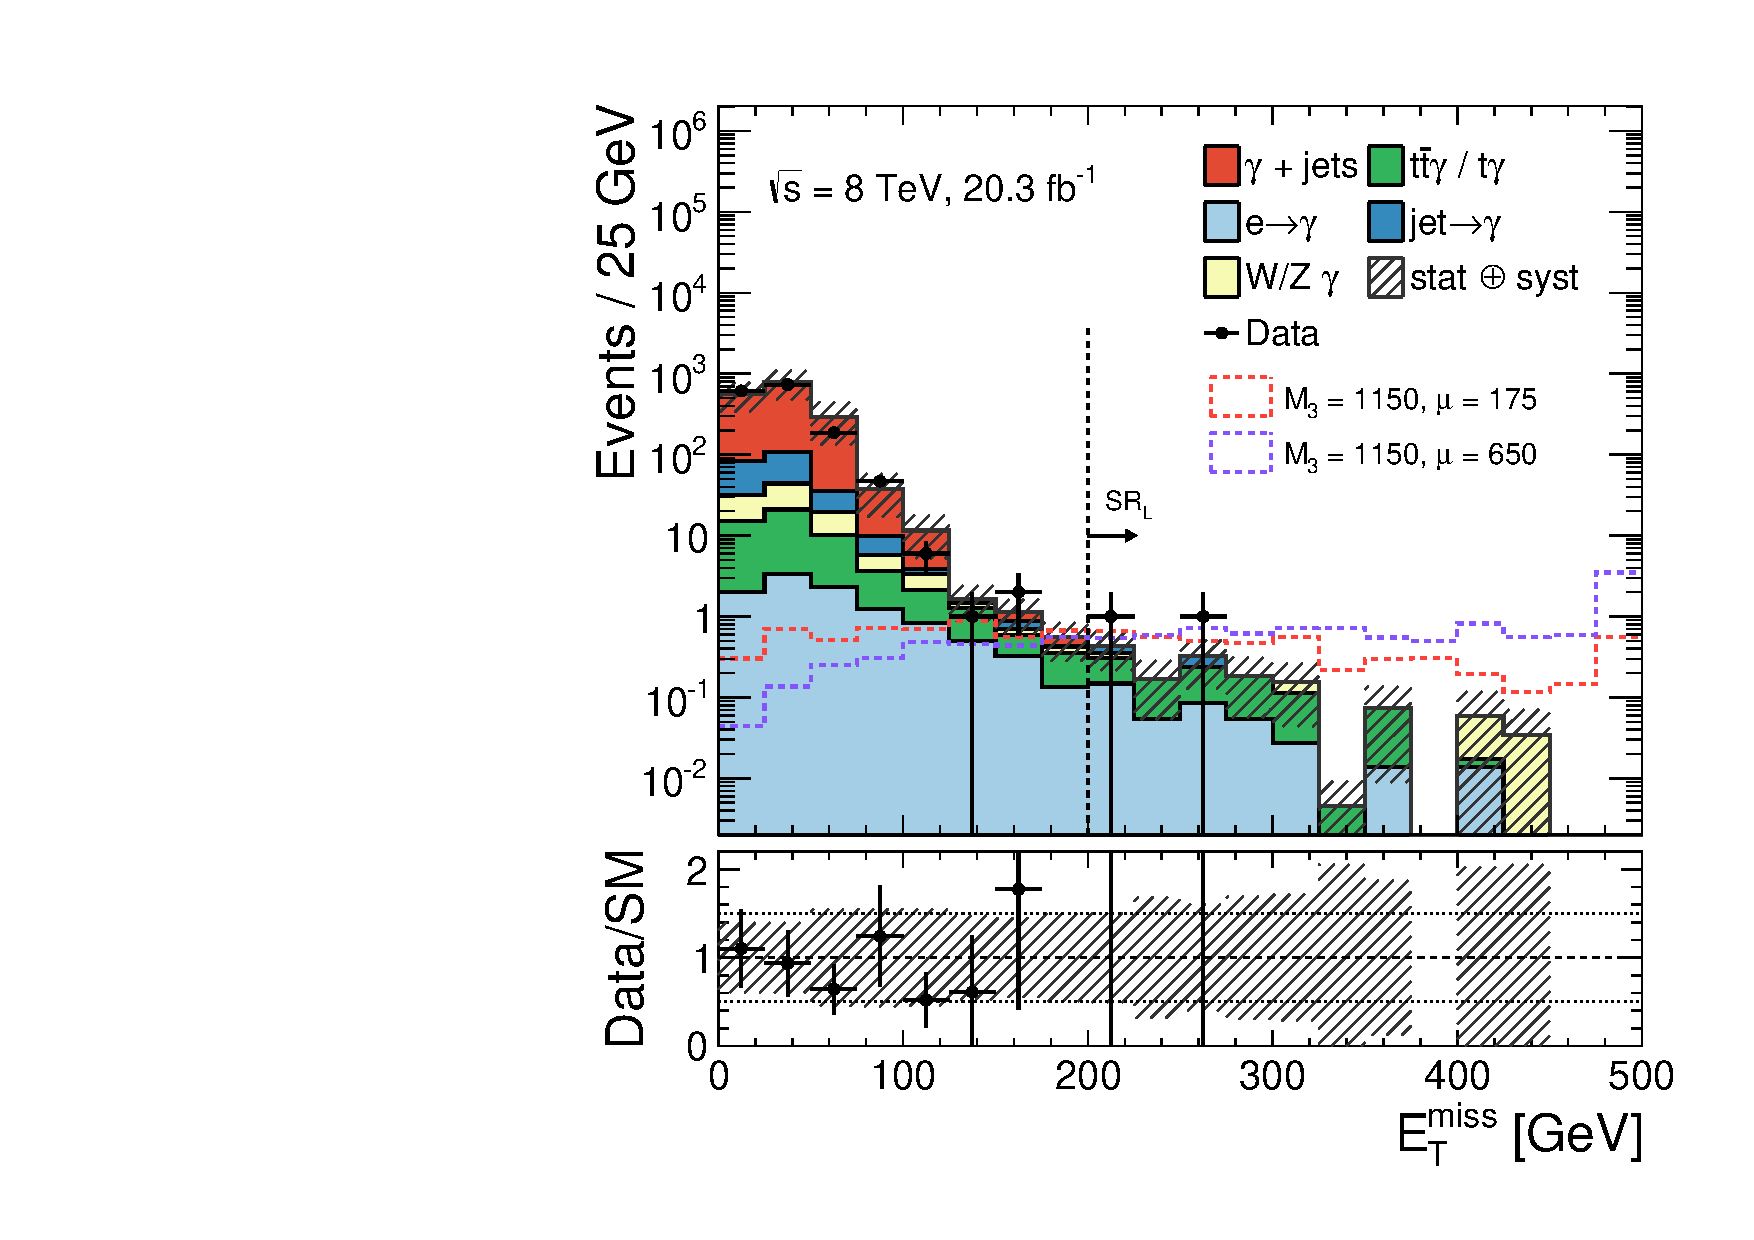
\includegraphics[width=0.49\textwidth]{plot_after_SRL_met_et}
  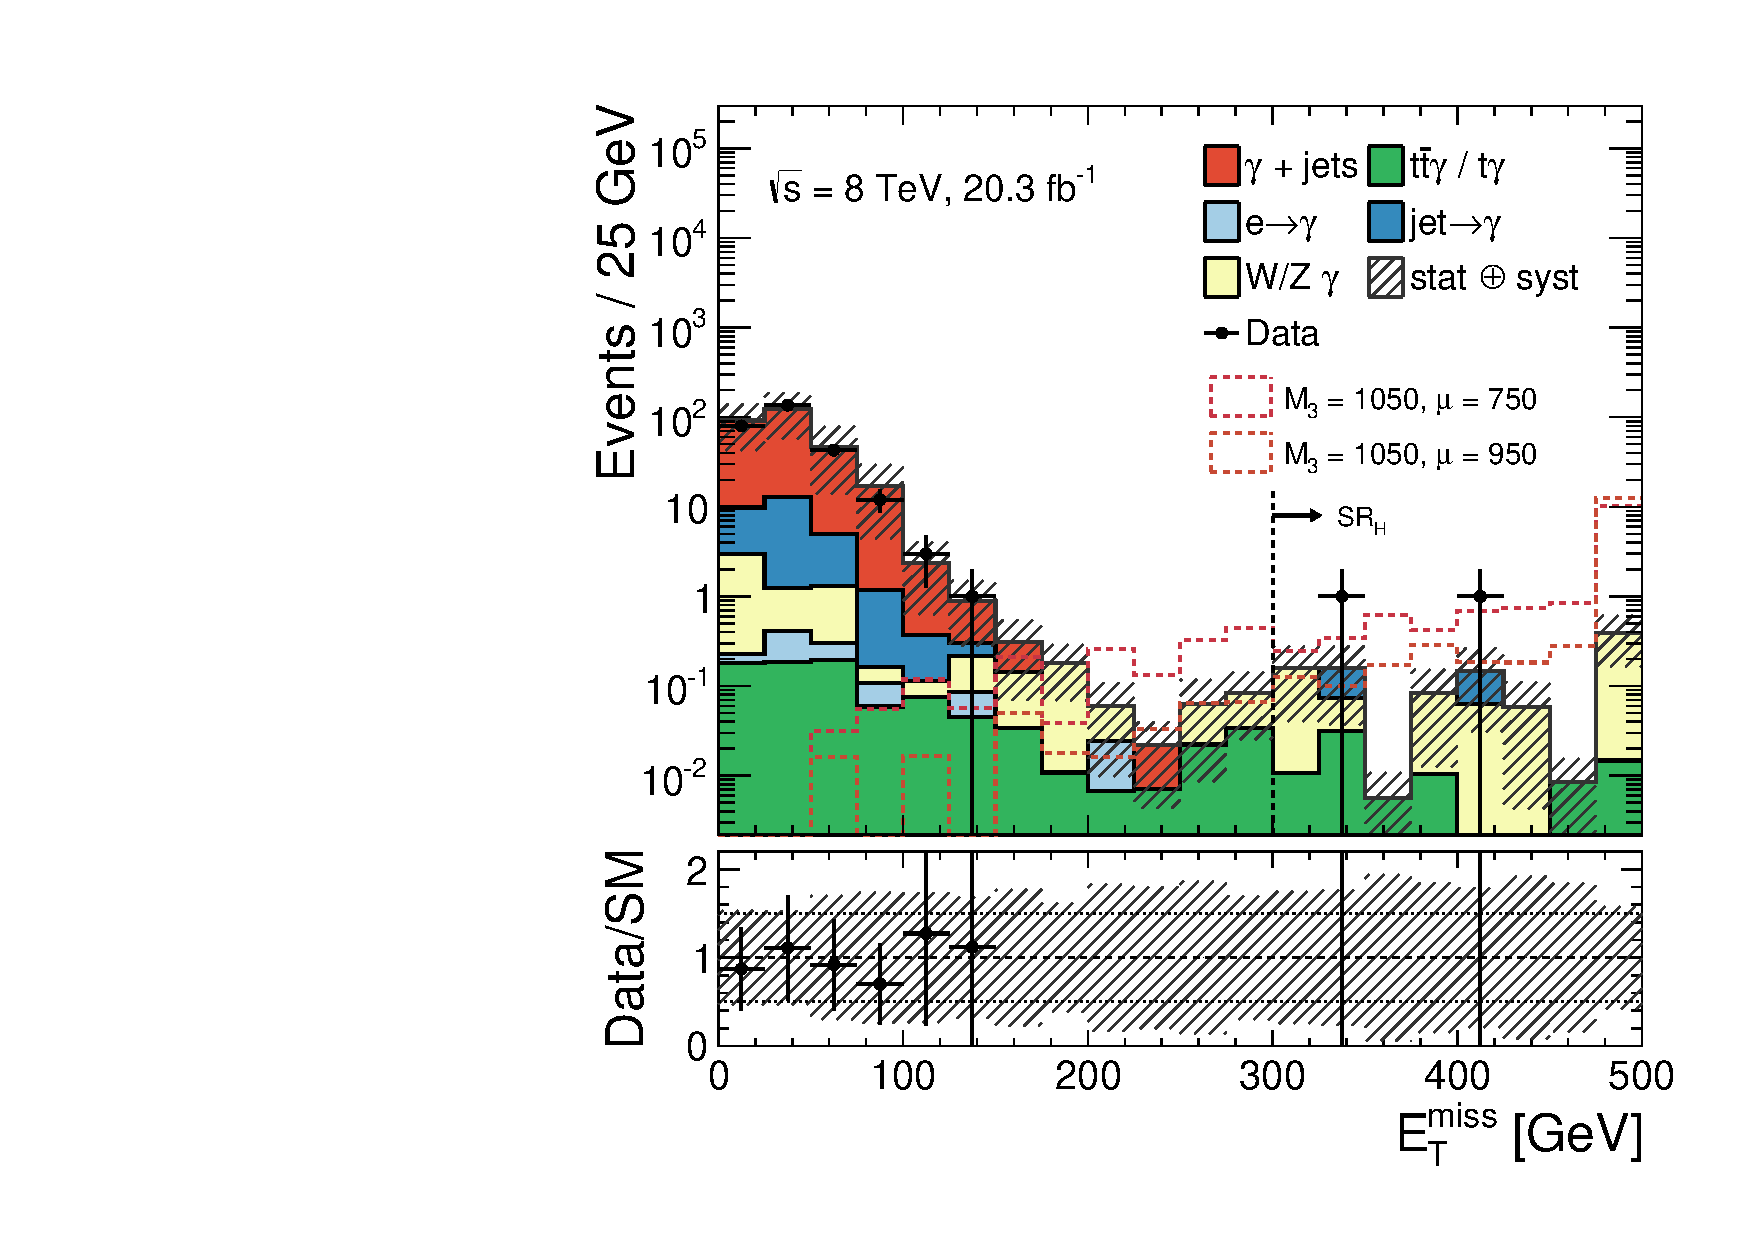
\includegraphics[width=0.49\textwidth]{plot_after_SRH_met_et}

  \caption{Distribución de {\met} comparando datos y el fondo esperado para la
    selección de la región {\SRL} (izquierda) y {\SRH} (derecha), sin el corte
    en {\met}. La distribución esperada para dos muestras de señal es también
    graficada para su comparación.}
  \label{fig:met_sr}

\end{figure}

Una comparación entre el número de eventos observado y esperado en cada una de las
regiones se presenta en la \cref{fig:fit_region_composition} a modo de resumen, donde
el panel inferior muestra el \emph{pull} de cada región. Se puede ver el buen acuerdo
tanto en las regiones de validación como en las de señal.


\begin{figure}[!htbp]
  \centering

  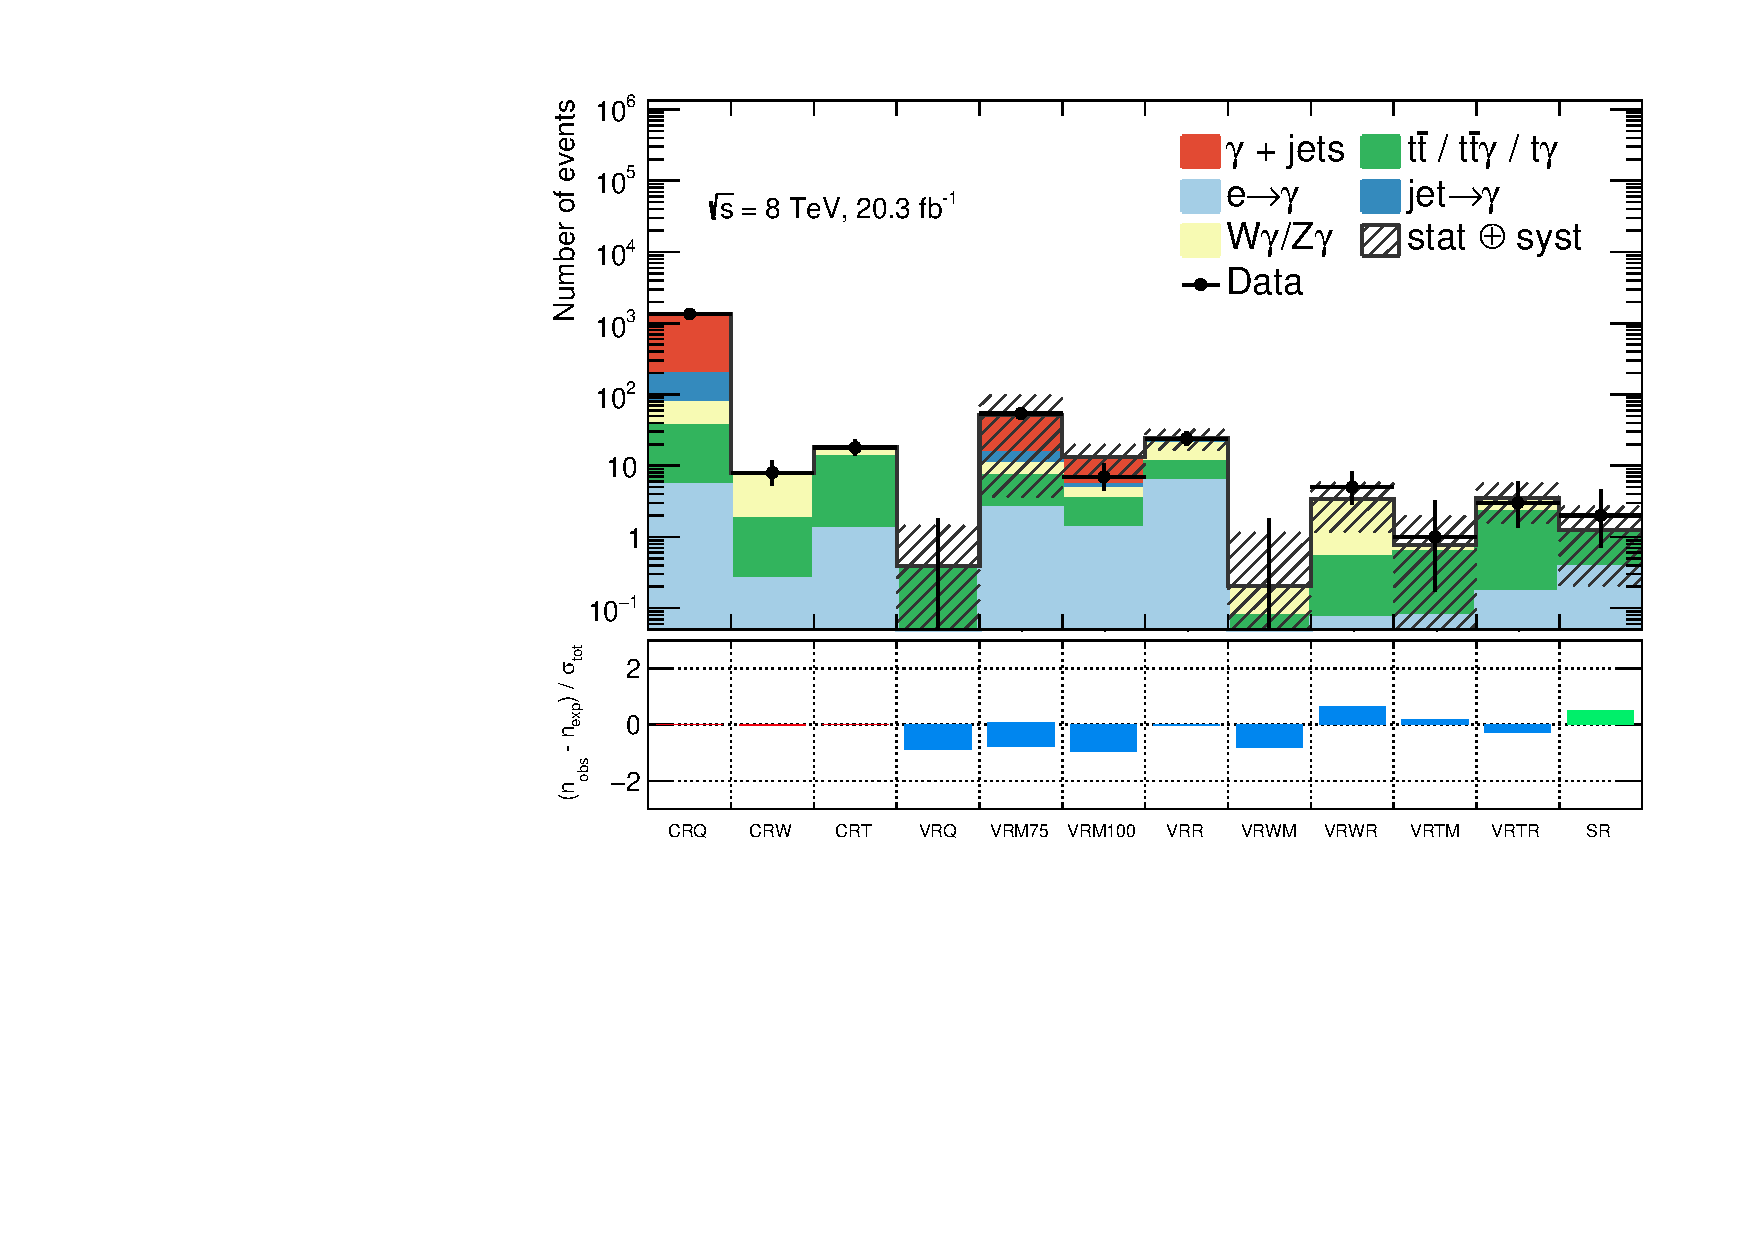
\includegraphics[width=0.9\textwidth]{histpull_SRL}
  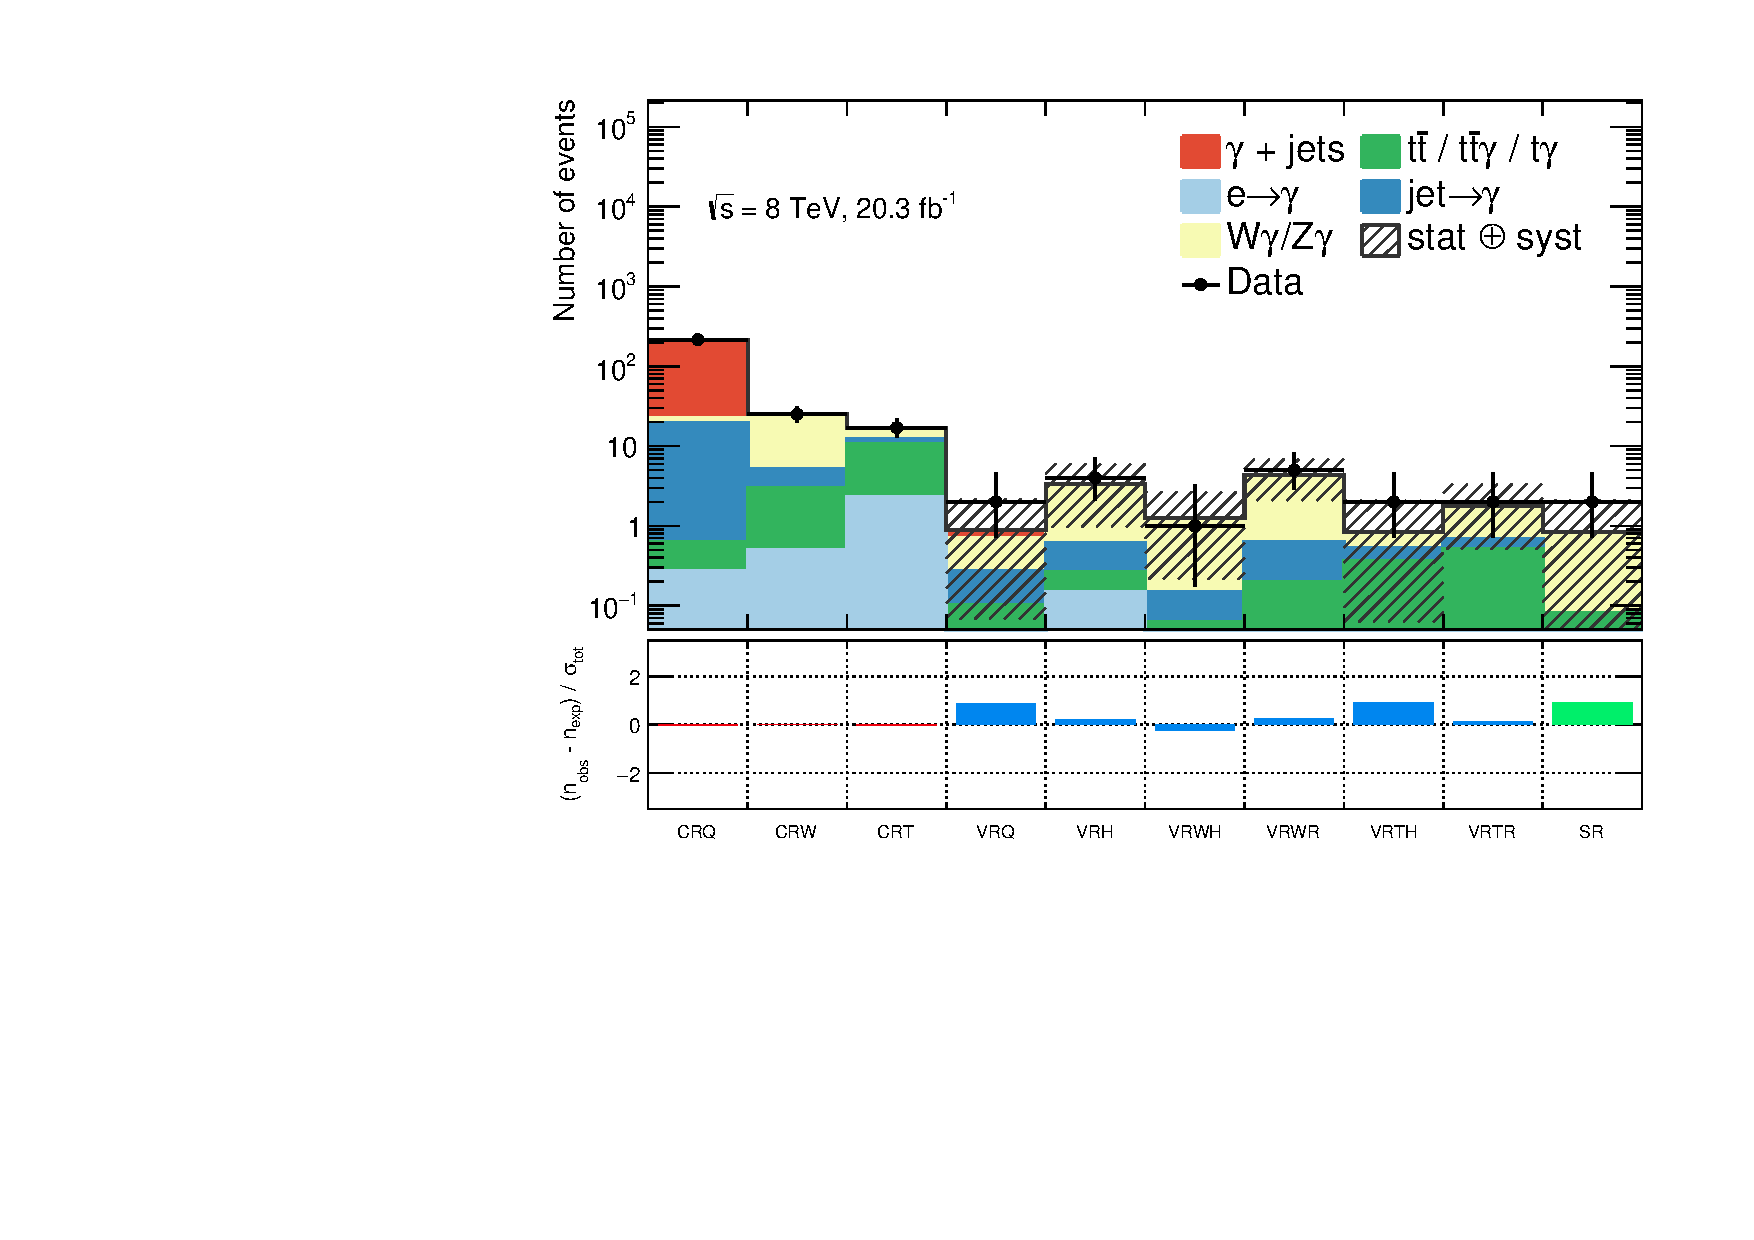
\includegraphics[width=0.9\textwidth]{histpull_SRH}

  \caption{Comparación entre el número de eventos observado y esperado en cada
    una de las regiones correspondientes a {\SRL} (arriba) y {\SRH} (abajo).}

  \label{fig:fit_region_composition}

\end{figure}


Las incertezas sistemáticas dominantes en el número total predicho de fondo en
cada SR, se presentan en \cref{tab:syst_srl,tab:syst_srh}.
Debido a que las incertezas individuales pueden estar correlacionadas y las
correlaciones negativas entre normalizaciones (representando el impacto de la
estadística en las CR en la incerteza total), la incerteza total no es
necesariamente la suma en cuadratura de las mismas. La incerteza estadística se
ilustra con el valor de la raíz cuadrada del número de eventos esperado con la
finalidad de mostrar el impacto relativo de la incerteza estadística con
respecto a la incerteza total del fondo. Las incertezas sistemáticas relativas
con respecto a las predicciones del fondo son del orden de 54\% (58\%) para
{\SRL} (\SRH). En {\SRL} las incertezas dominantes provienen de la normalización
y de las incertezas teóricas del fondo de {\ttgam}, seguidas por la incerteza en
la escala de energía de los jets. En {\SRH}, las
incertezas están dominadas por las incertezas teóricas del fondo {\zgam} y
{\gjet}, y la incerteza en la normalización del fondo {\wgam}.


\begin{table}[!htbp]
  \centering

  \caption{Resumen de las incertezas sistemáticas dominantes en la estimación del fondo total
    en {\SRL} y {\SRH}. Notar que las incertezas individuales pueden estar correlacionadas, y la incerteza
    total no es necesariamente la suma en cuadratura de estas. Los porcentajes muestran el tamaño
    de la incerteza relativo al fondo esperado total.}
  \label{tab:syst_srl}

  \begin{tabularx}{\textwidth}{z{5cm}RR}
\hline
{\bf Incertezas}                                    & {\SRL}   & {\SRH}          \\
\hline
Eventos esperados SM             &  $1.27$       & $0.84$ \\
\hline
Incerteza estadística total $(\sqrt{N})$              & $\pm 1.13$     & $\pm 0.92$  \\
Incerteza sistemática total               & $\pm 0.43\ [34.18\%] $             & $\pm 0.38\ [45.27\%] $ \\
\hline
{\tgam}         & $\pm 0.36\ [28.0\%] $      & $\pm 0.02\ [1.8\%] $  \\
$\mu_{T}$         & $\pm 0.35\ [27.7\%] $       & $\pm 0.04\ [4.4\%] $ \\
%%$\gamma_\mathrm{SR}$        & $\pm 0.22\ [17.4\%] $       & $\pm 0.20\ [24.3\%] $ \\
JES         & $\pm 0.21\ [16.5\%] $       & $\pm 0.03\ [4.0\%] $ \\
Teoría {\wgam}         & $\pm 0.09\ [7.3\%] $       & $\pm 0.21\ [25.1\%] $ \\
$\mu_{W}$        & $\pm 0.08\ [6.7\%] $       & $\pm 0.17\ [20.5\%] $\\
Estimación ${j\to\gamma}$         & $\pm 0.08\ [6.3\%] $       & $\pm 0.08\ [9.5\%] $ \\
Estimación ${e\to\gamma}$         & $\pm 0.07\ [5.7\%] $       & - \\
JER         & $\pm 0.06\ [4.3\%] $      & $\pm 0.04\ [4.8\%] $ \\
Teoría ${Z\gamma}$         & $\pm 0.03\ [2.7\%] $       & $\pm 0.21\ [25.4\%] $ \\
EGMAT         & $\pm 0.03\ [2.2\%] $       & $\pm 0.04\ [4.5\%] $ \\
EGRES         & $\pm 0.03\ [2.0\%] $       & $\pm 0.05\ [5.8\%] $\\
Término \emph{soft} de  {\met}         & $\pm 0.02\ [1.7\%] $       & - \\ %% SCALEST
Corrección \emph{pile-up}         & $\pm 0.01\ [0.71\%] $       & $\pm 0.10\ [11.9\%] $ \\
RESOST         & $\pm 0.00\ [0.35\%] $      & $\pm 0.04\ [4.5\%] $ \\
${t\gamma}$         & $\pm 0.00\ [0.34\%] $      & $0.00\ [0.22\%] $  \\
Eficiencia fotones         & $\pm 0.00\ [0.06\%] $       & $\pm 0.00\ [0.40\%] $\\ % PHEFF
$\mu_{Q}$         & $\pm 0.00\ [0.02\%] $       & - \\
Teoria ${\gamma j}$         & $\pm 0.00\ [0.02\%] $ & -      \\
%% MMS      &   - & $\pm 0.01\ [1.3\%] $       \\ %MMS
%% MID      &   - & $\pm 0.01\ [1.3\%] $       \\ %MID
\hline
\end{tabularx}

\end{table}

%% \begin{table}[!htbp]
%%   \centering

%%   \caption{Resumen de las incertezas sistematicas dominantes en la estimacion del fondo total
%%     en {\SRH}. Notar que las incertezas individuales pueden estar correlacionados, y la incerteza
%%     total no es necesariamente la suma en cuadratura de estas. Los porcentajes muestran el tamano
%%     de la incerteza relativo al fondo esperado total.}
%%   \label{tab:syst_srh}

%%   \begin{tabularx}{\textwidth}{LR}
\hline
{\bf Incertezas}                                    & {\SRH}            \\
\hline
Eventos esperados SM             &  $0.84$       \\
\noalign{\smallskip}\hline\noalign{\smallskip}
Incerteza estadística total $(\sqrt{N_{\rm SM}})$              & $\pm 0.92$       \\
Incerteza sistemática total               & $\pm 0.38\ [45.27\%] $             \\
\hline
$\alpha_{Z\gamma}$         & $\pm 0.21\ [25.4\%] $       \\
$\alpha_{\wgam}$         & $\pm 0.21\ [25.1\%] $       \\
$\gamma_\mathrm{SR}$         & $\pm 0.20\ [24.3\%] $       \\
$\mu_{W}$         & $\pm 0.17\ [20.5\%] $       \\
$\alpha_\mathrm{PRW}$         & $\pm 0.10\ [11.9\%] $       \\
$\alpha_\mathrm{JFAKE}$         & $\pm 0.08\ [9.5\%] $       \\
$\alpha_\mathrm{EGRES}$         & $\pm 0.05\ [5.8\%] $       \\
$\alpha_\mathrm{JER}$         & $\pm 0.04\ [4.8\%] $       \\
%% $\alpha_\mathrm{RESOST}$         & $\pm 0.04\ [4.5\%] $       \\
%% $\alpha_\mathrm{EGMAT}$         & $\pm 0.04\ [4.5\%] $       \\
%% $\mu_{T}$         & $\pm 0.04\ [4.4\%] $       \\
%% $\alpha_\mathrm{JES}$         & $\pm 0.03\ [4.0\%] $       \\
%% $\alpha_{\tgam}$         & $\pm 0.02\ [1.8\%] $       \\
%% $\alpha_\mathrm{MMS}$         & $\pm 0.01\ [1.3\%] $       \\
%% $\alpha_\mathrm{MID}$         & $\pm 0.01\ [1.3\%] $       \\
%% $\alpha_\mathrm{PHEFF}$         & $\pm 0.00\ [0.40\%] $       \\
%% $\alpha_{t\gamma}$         & $\pm 0.00\ [0.22\%] $       \\
\hline
\end{tabularx}


%% \end{table}


\subsection{Eventos en las regiones de señal}

Solo dos eventos pasan la
selección de cada una de las regiones de señal. Un esquema del detector y las
se\~nales dejadas por los distintos objetos en el mismo puede verse en las
\cref{fig:evdisplay_srl} para los dos eventos observados en la {\SRL} y en las
\cref{fig:evdisplay_srh} para los dos eventos en la {\SRH}.

Las visualizaciones de los eventos es generada con
\textsc{Atlantis}\cite{atlantis}.
En la parte superior izquierda se puede ver el corte transversal del detector
junto con el corte transversal en el panel inferior. En estas vistas se presentan
los depósitos de energía en los calorímetros en color amarillo. Los conos de
distintos colores representan los jets reconstruidos... \hl{seguir}



\begin{figure}[!htbp]
  \begin{center}

    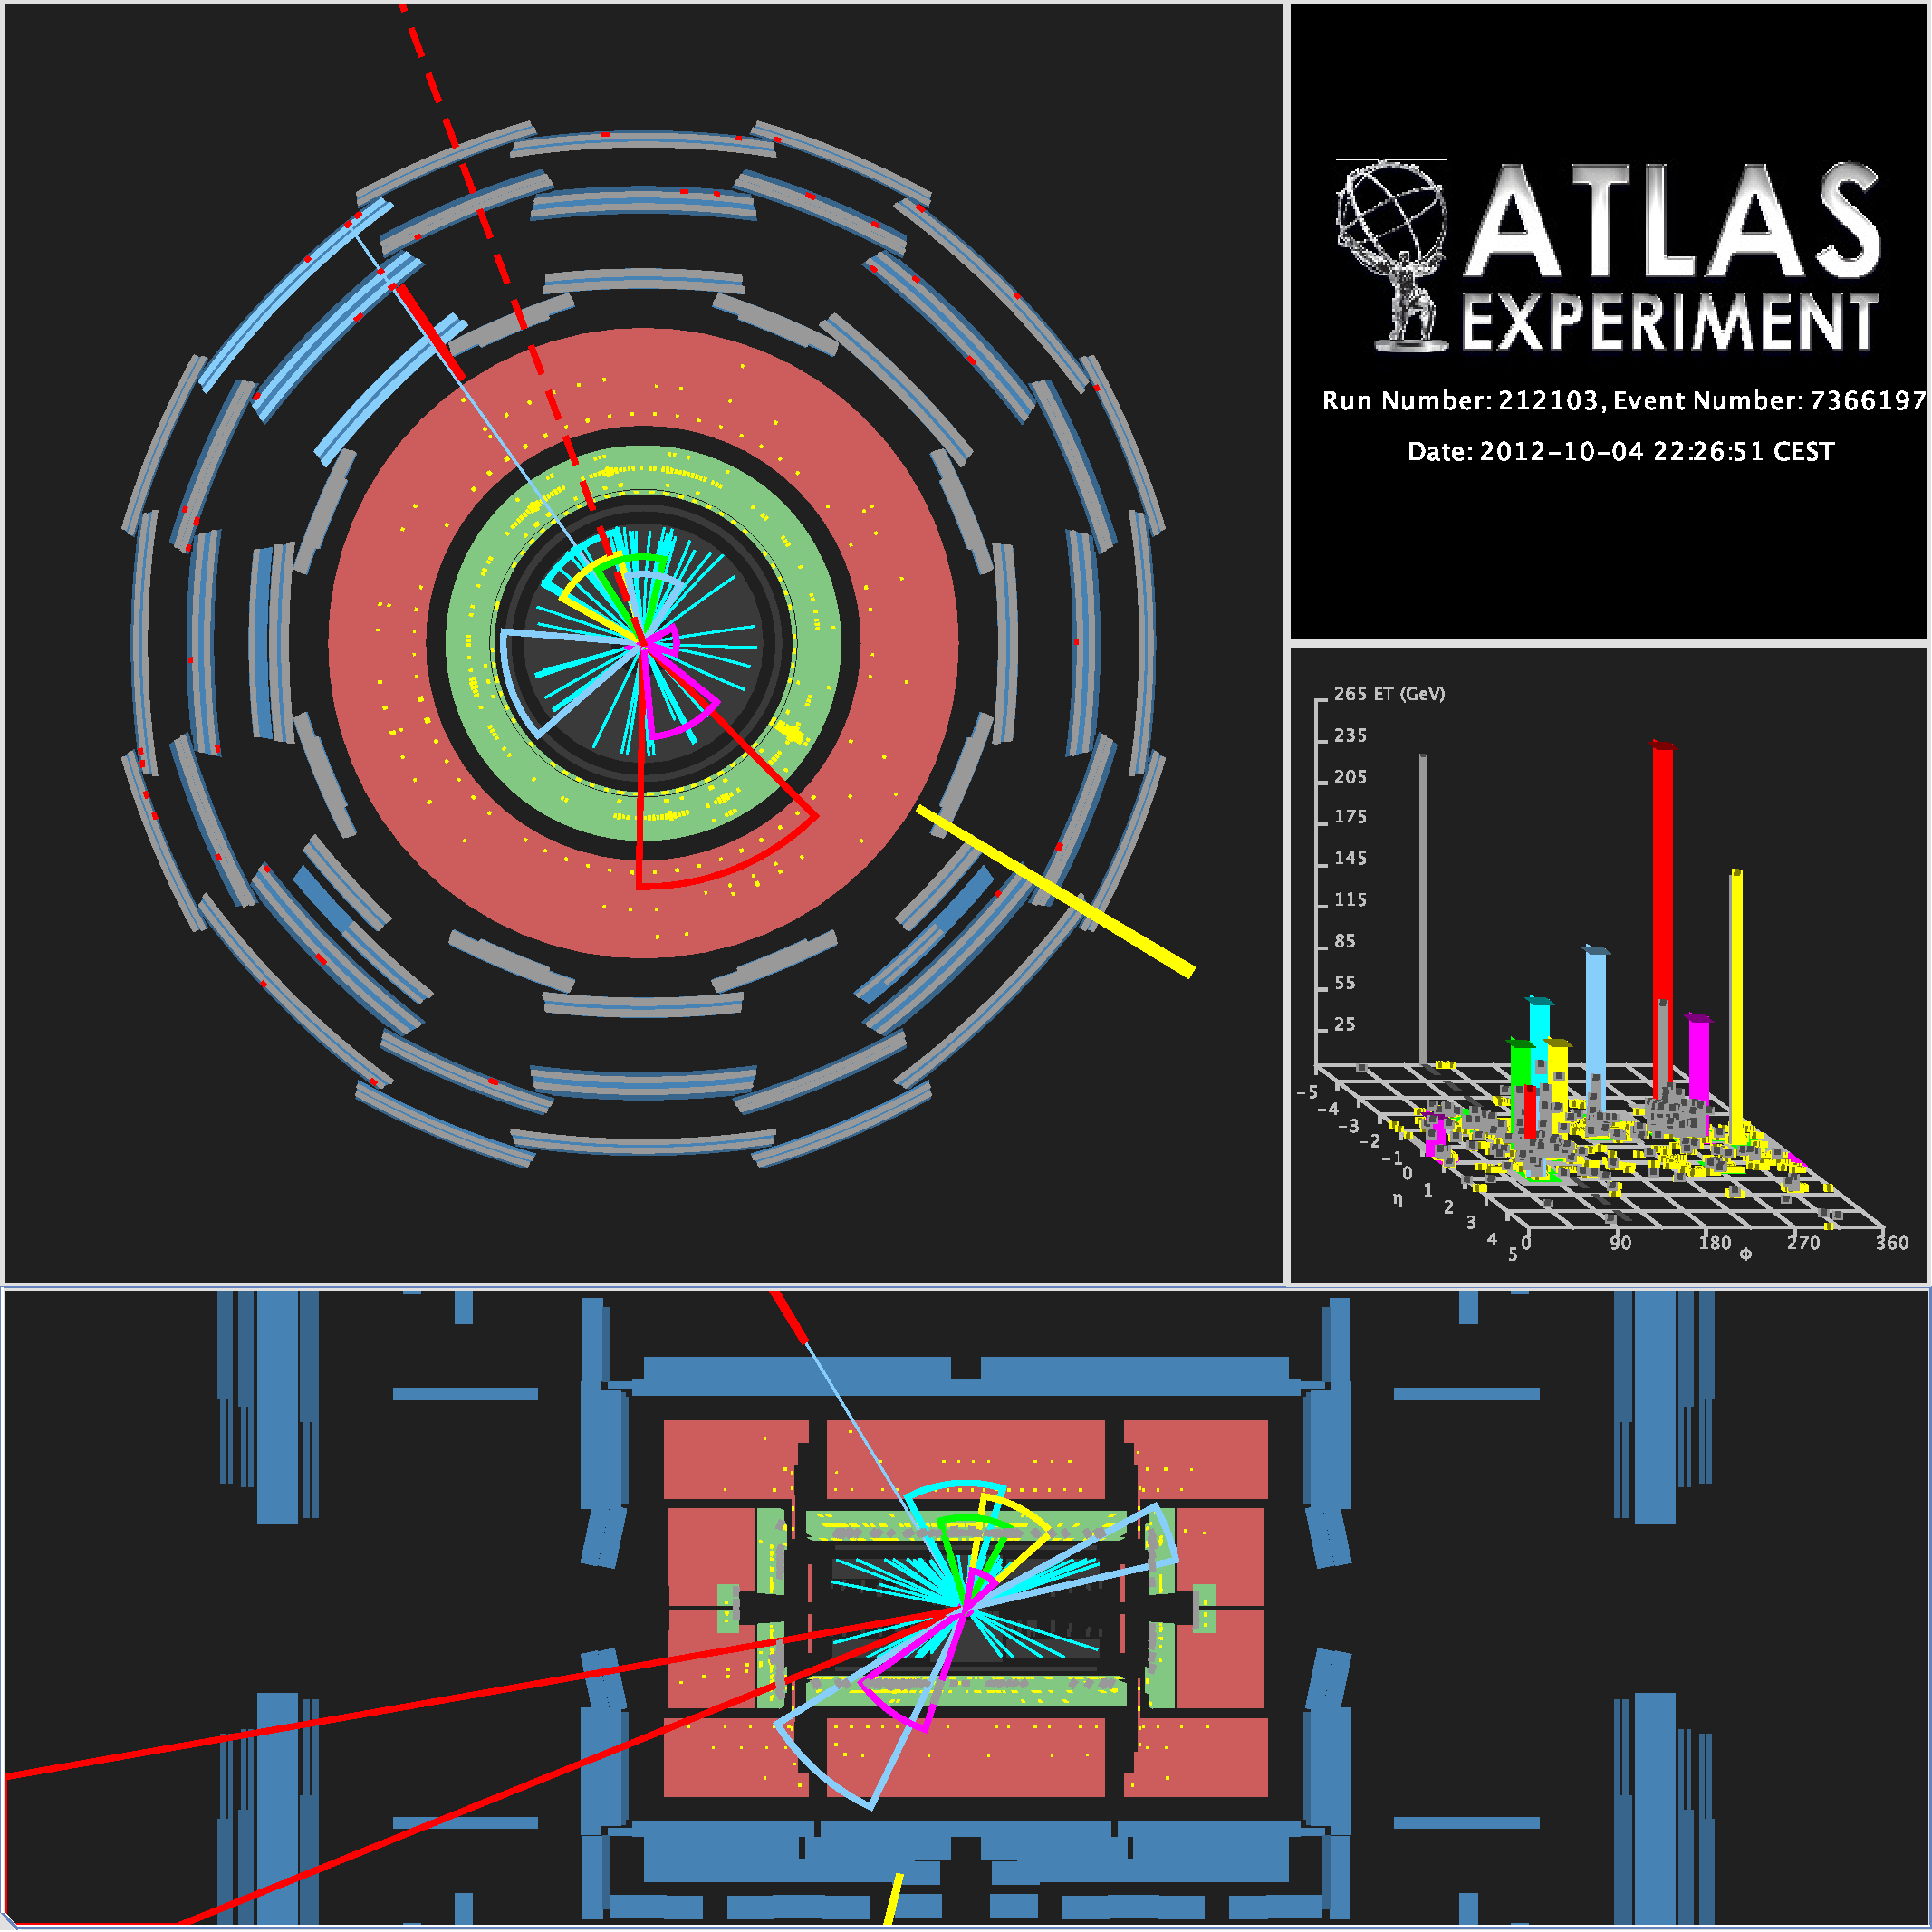
\includegraphics[height=0.45\textheight]{EvtDisplay_212103_73661974}

    \vspace{1cm}

    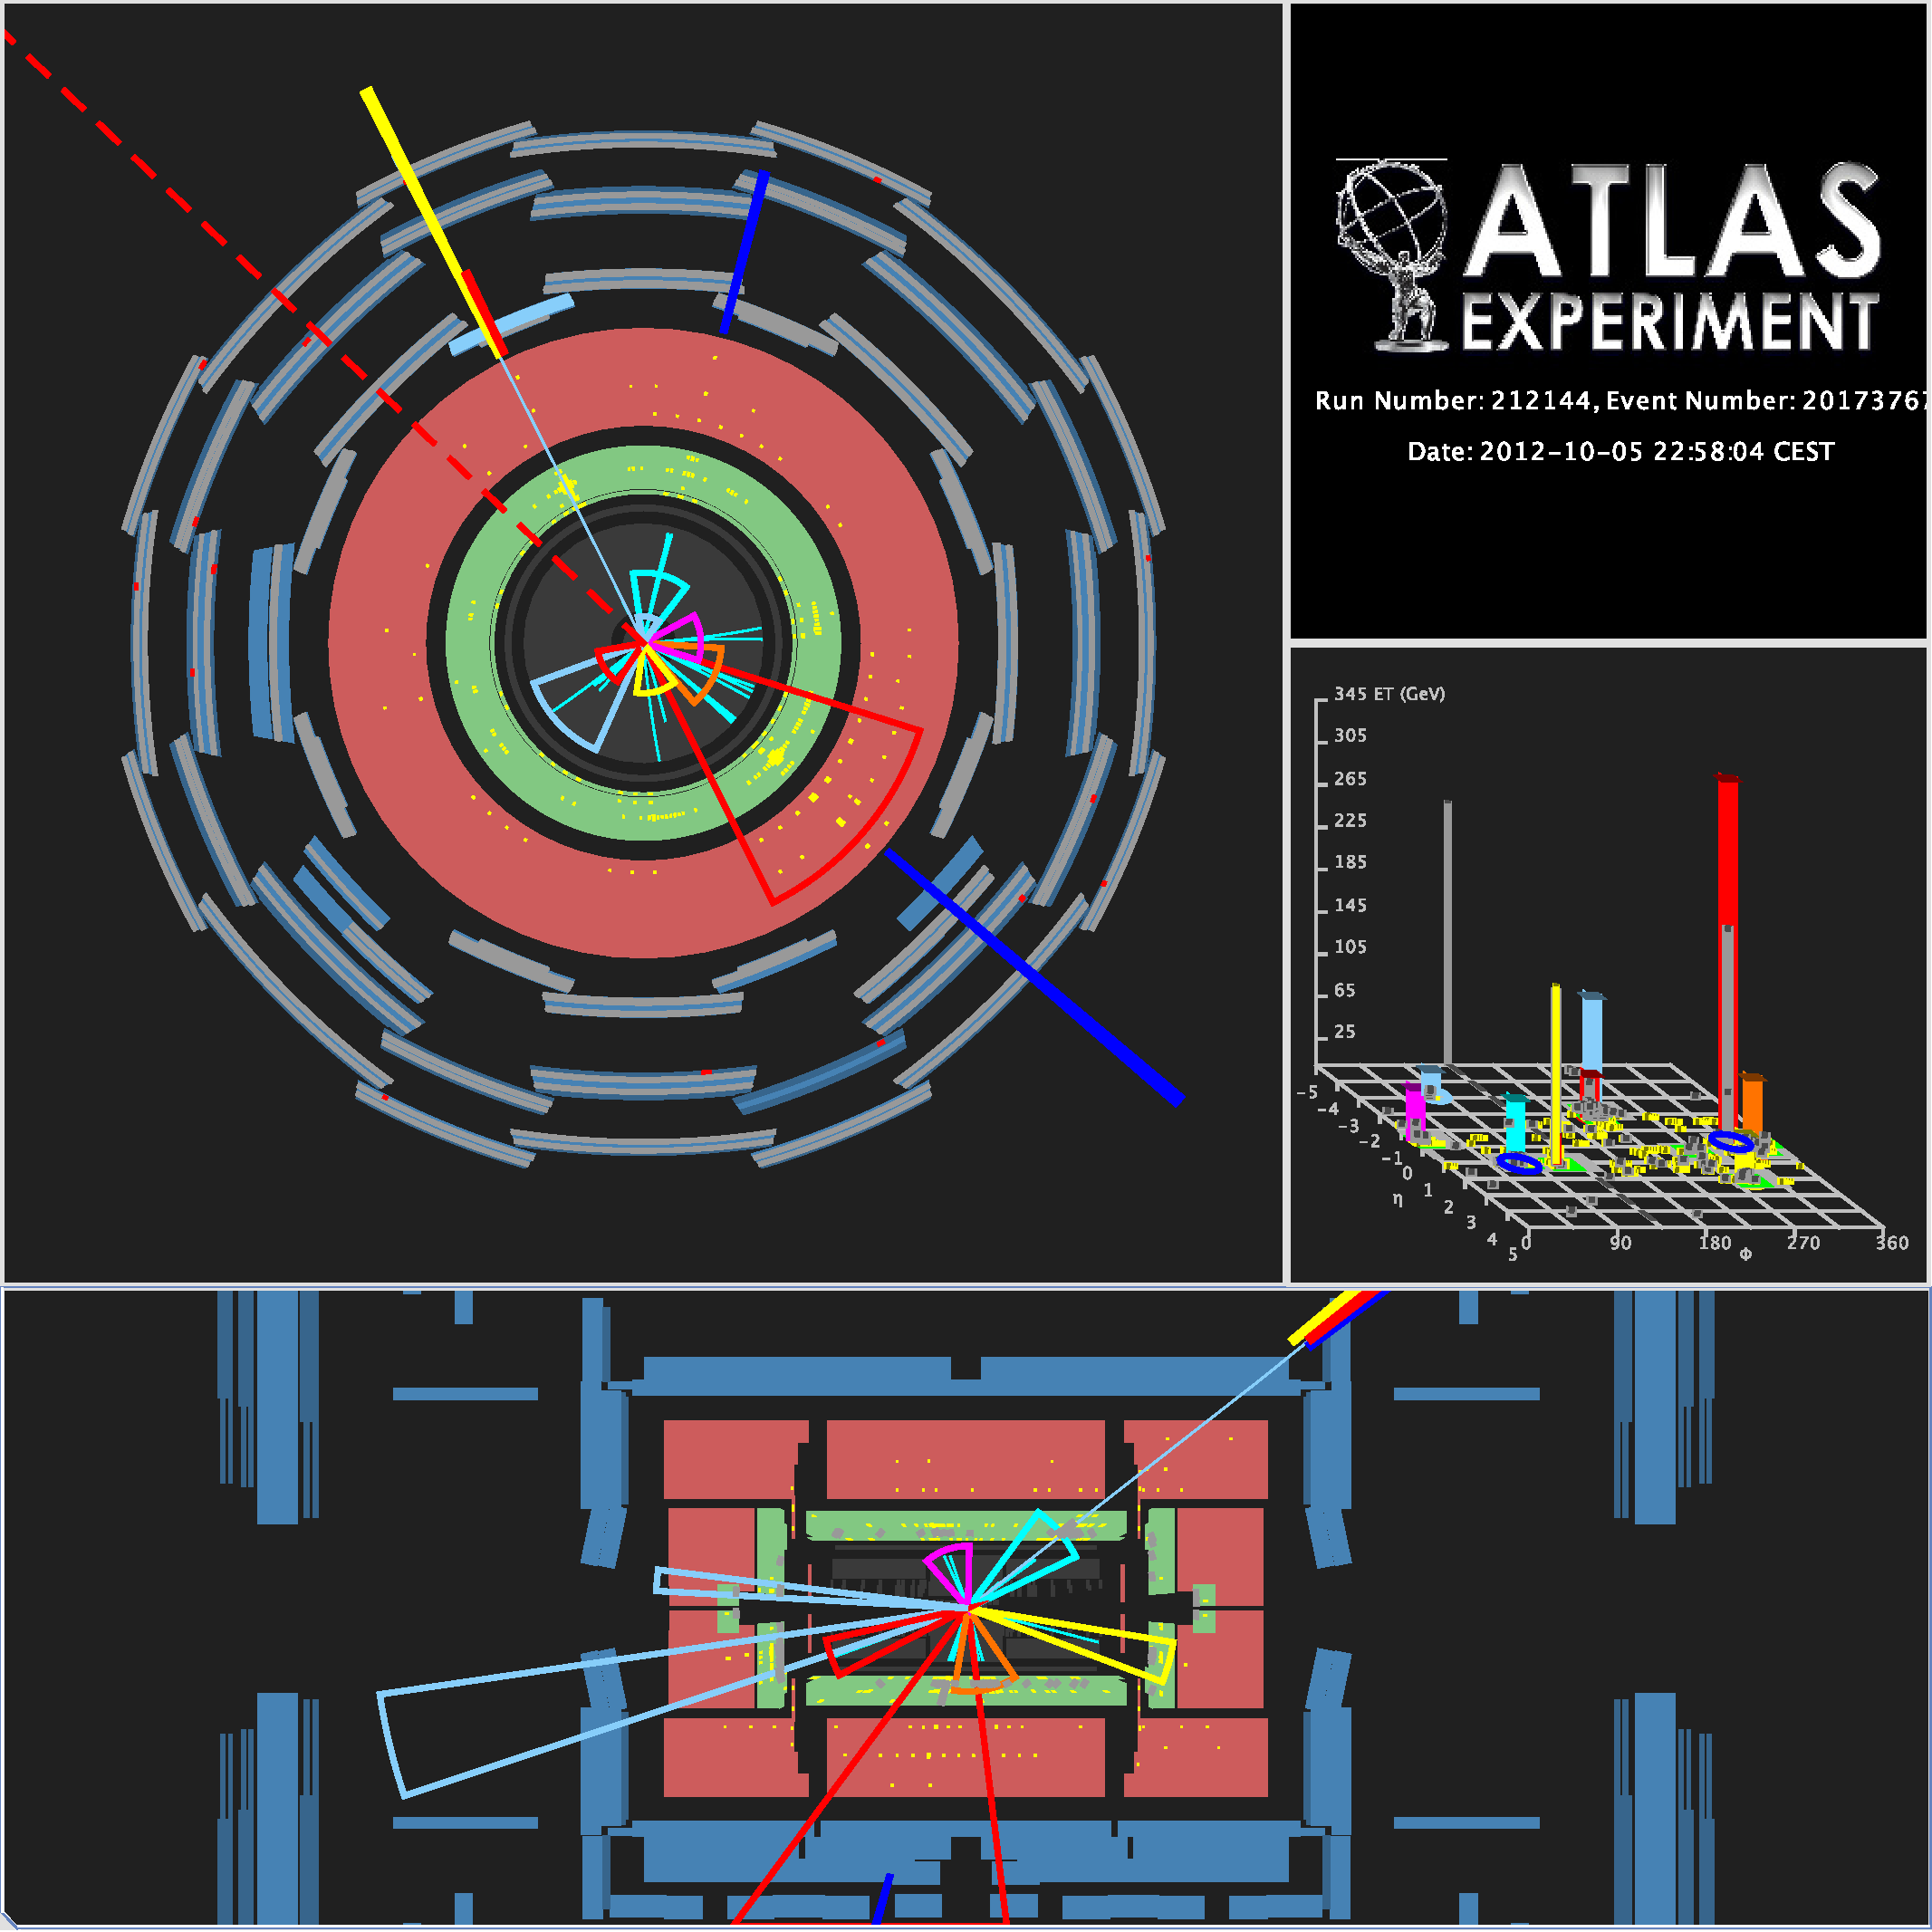
\includegraphics[height=0.45\textheight]{EvtDisplay_212144_201737678}

    \caption{Visualización de los dos eventos que sobreviven la selección de {\SRL}. Ver detalles en el texto.}
    \label{fig:evdisplay_srl}
  \end{center}
\end{figure}


\begin{figure}[!htbp]
  \begin{center}

    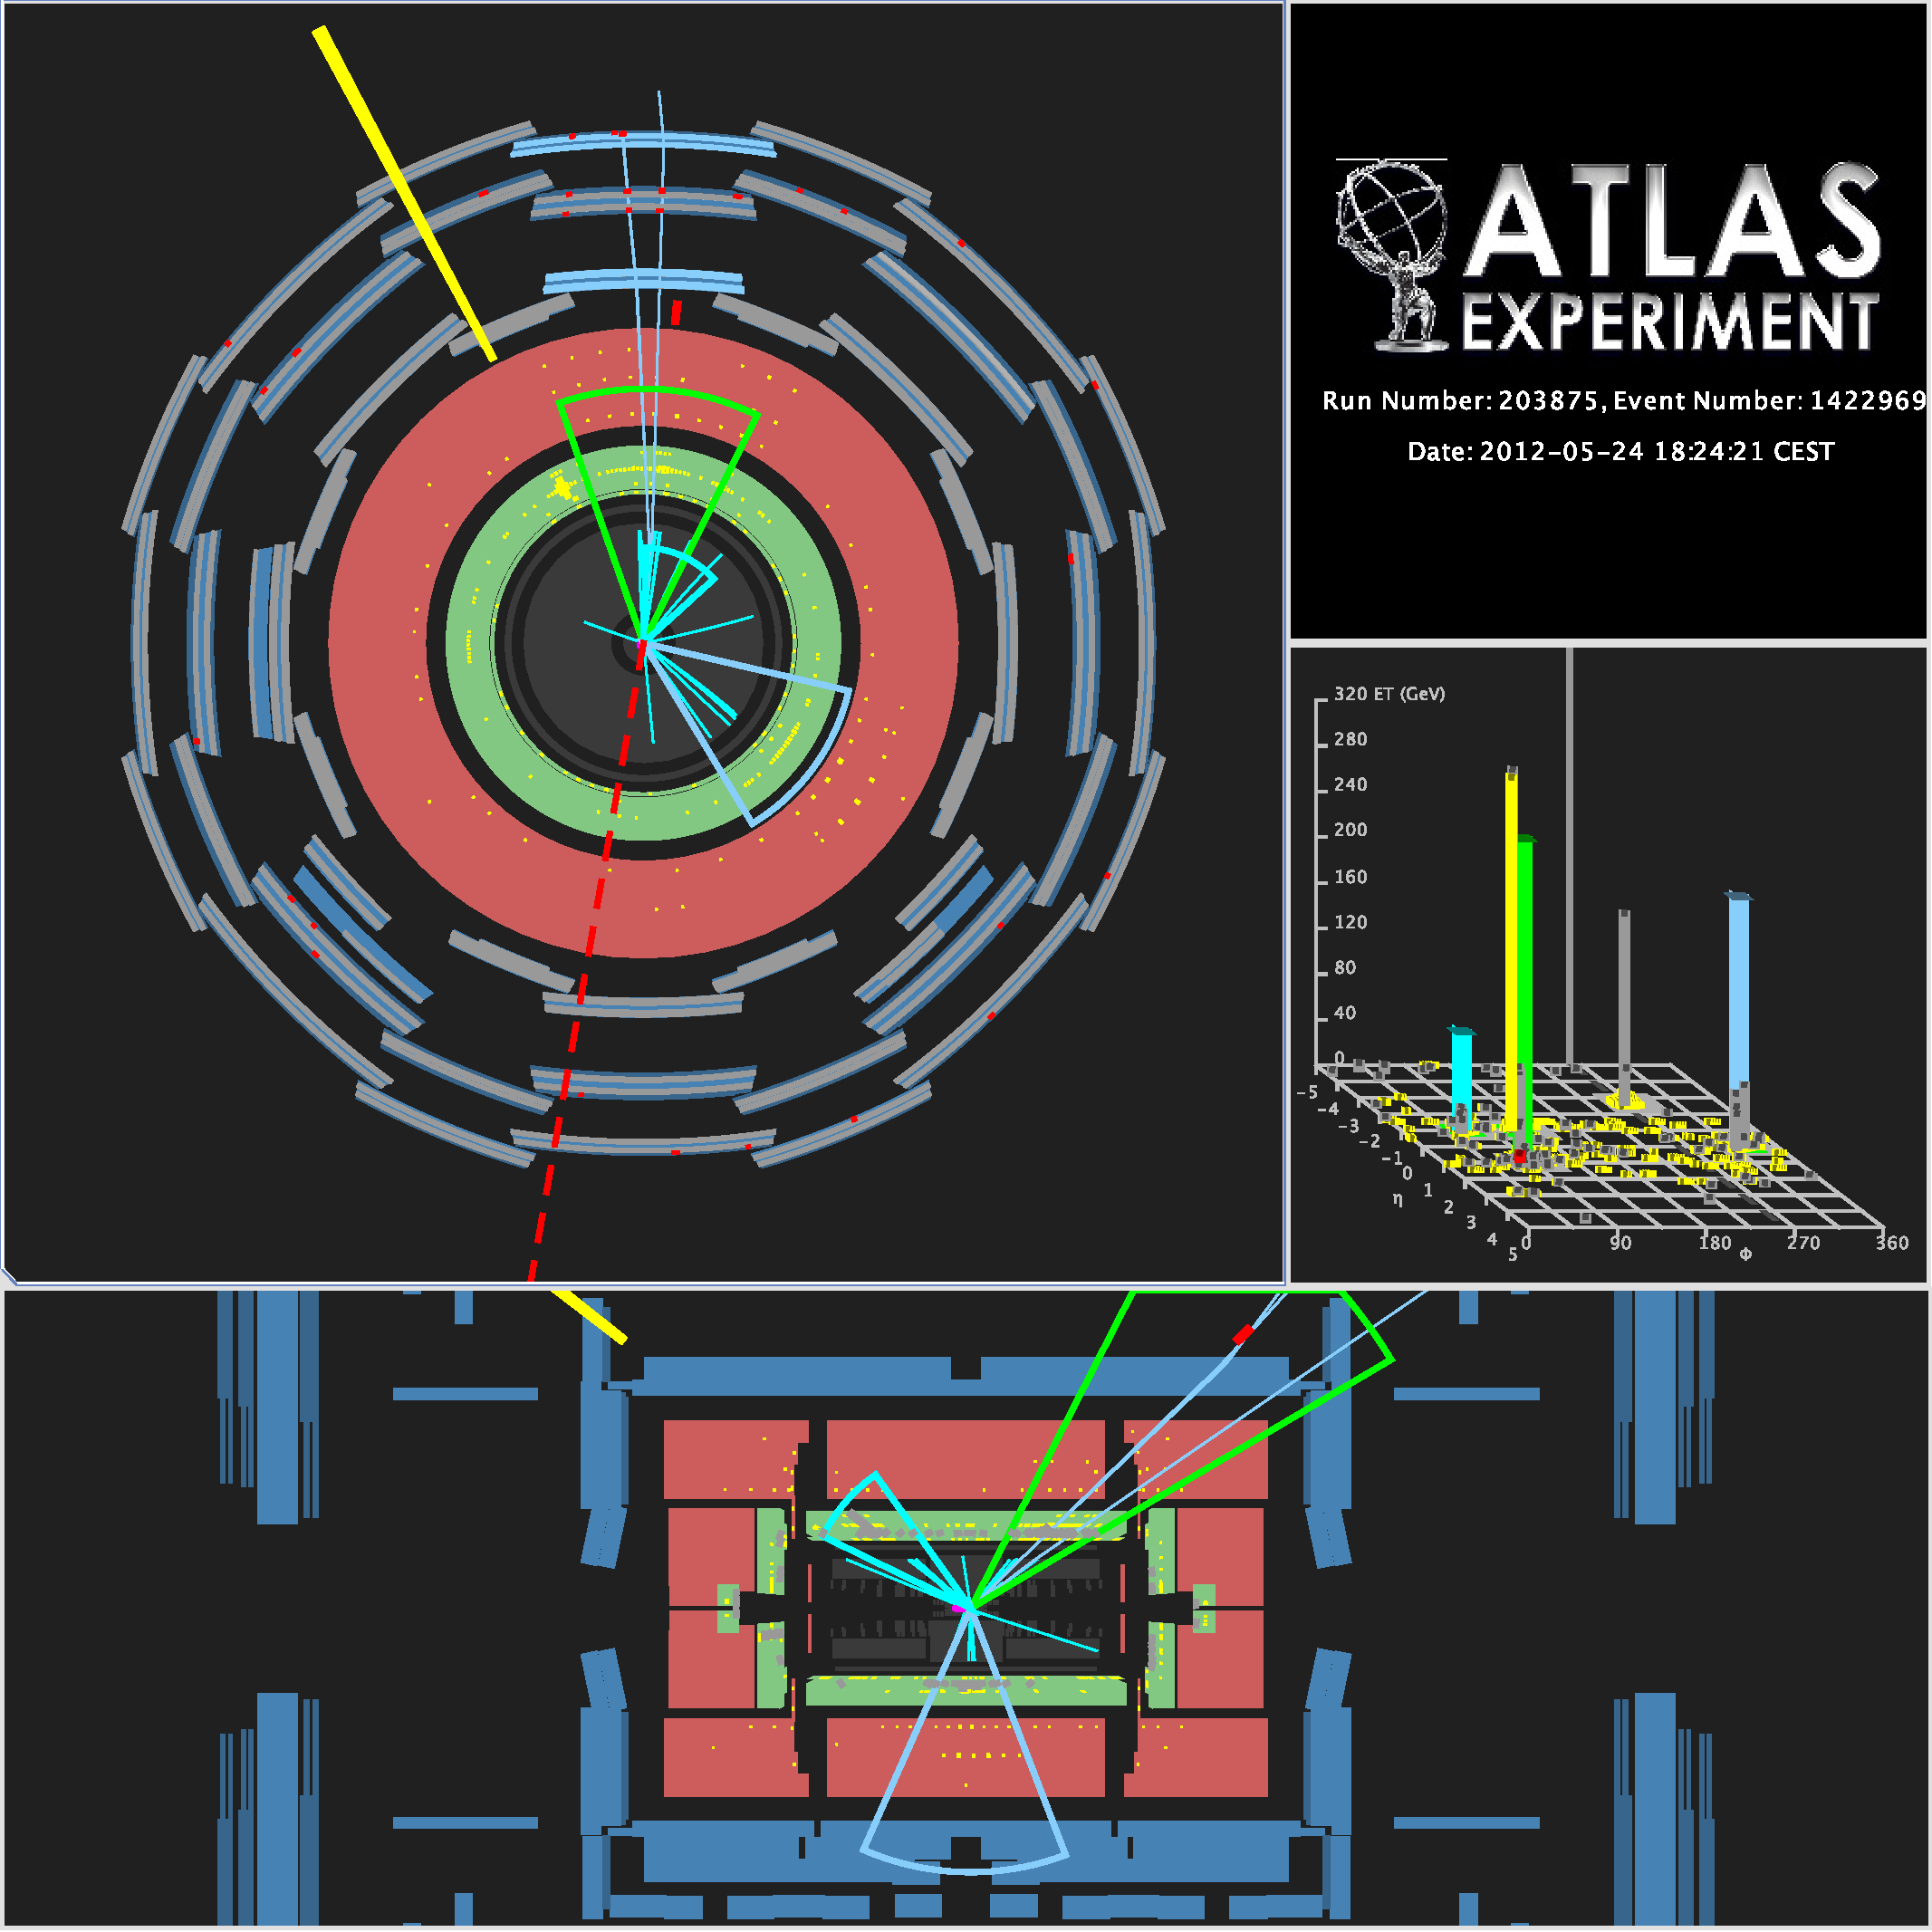
\includegraphics[height=0.45\textheight]{EvtDisplay_203875_14229699}

    \vspace{1cm}

    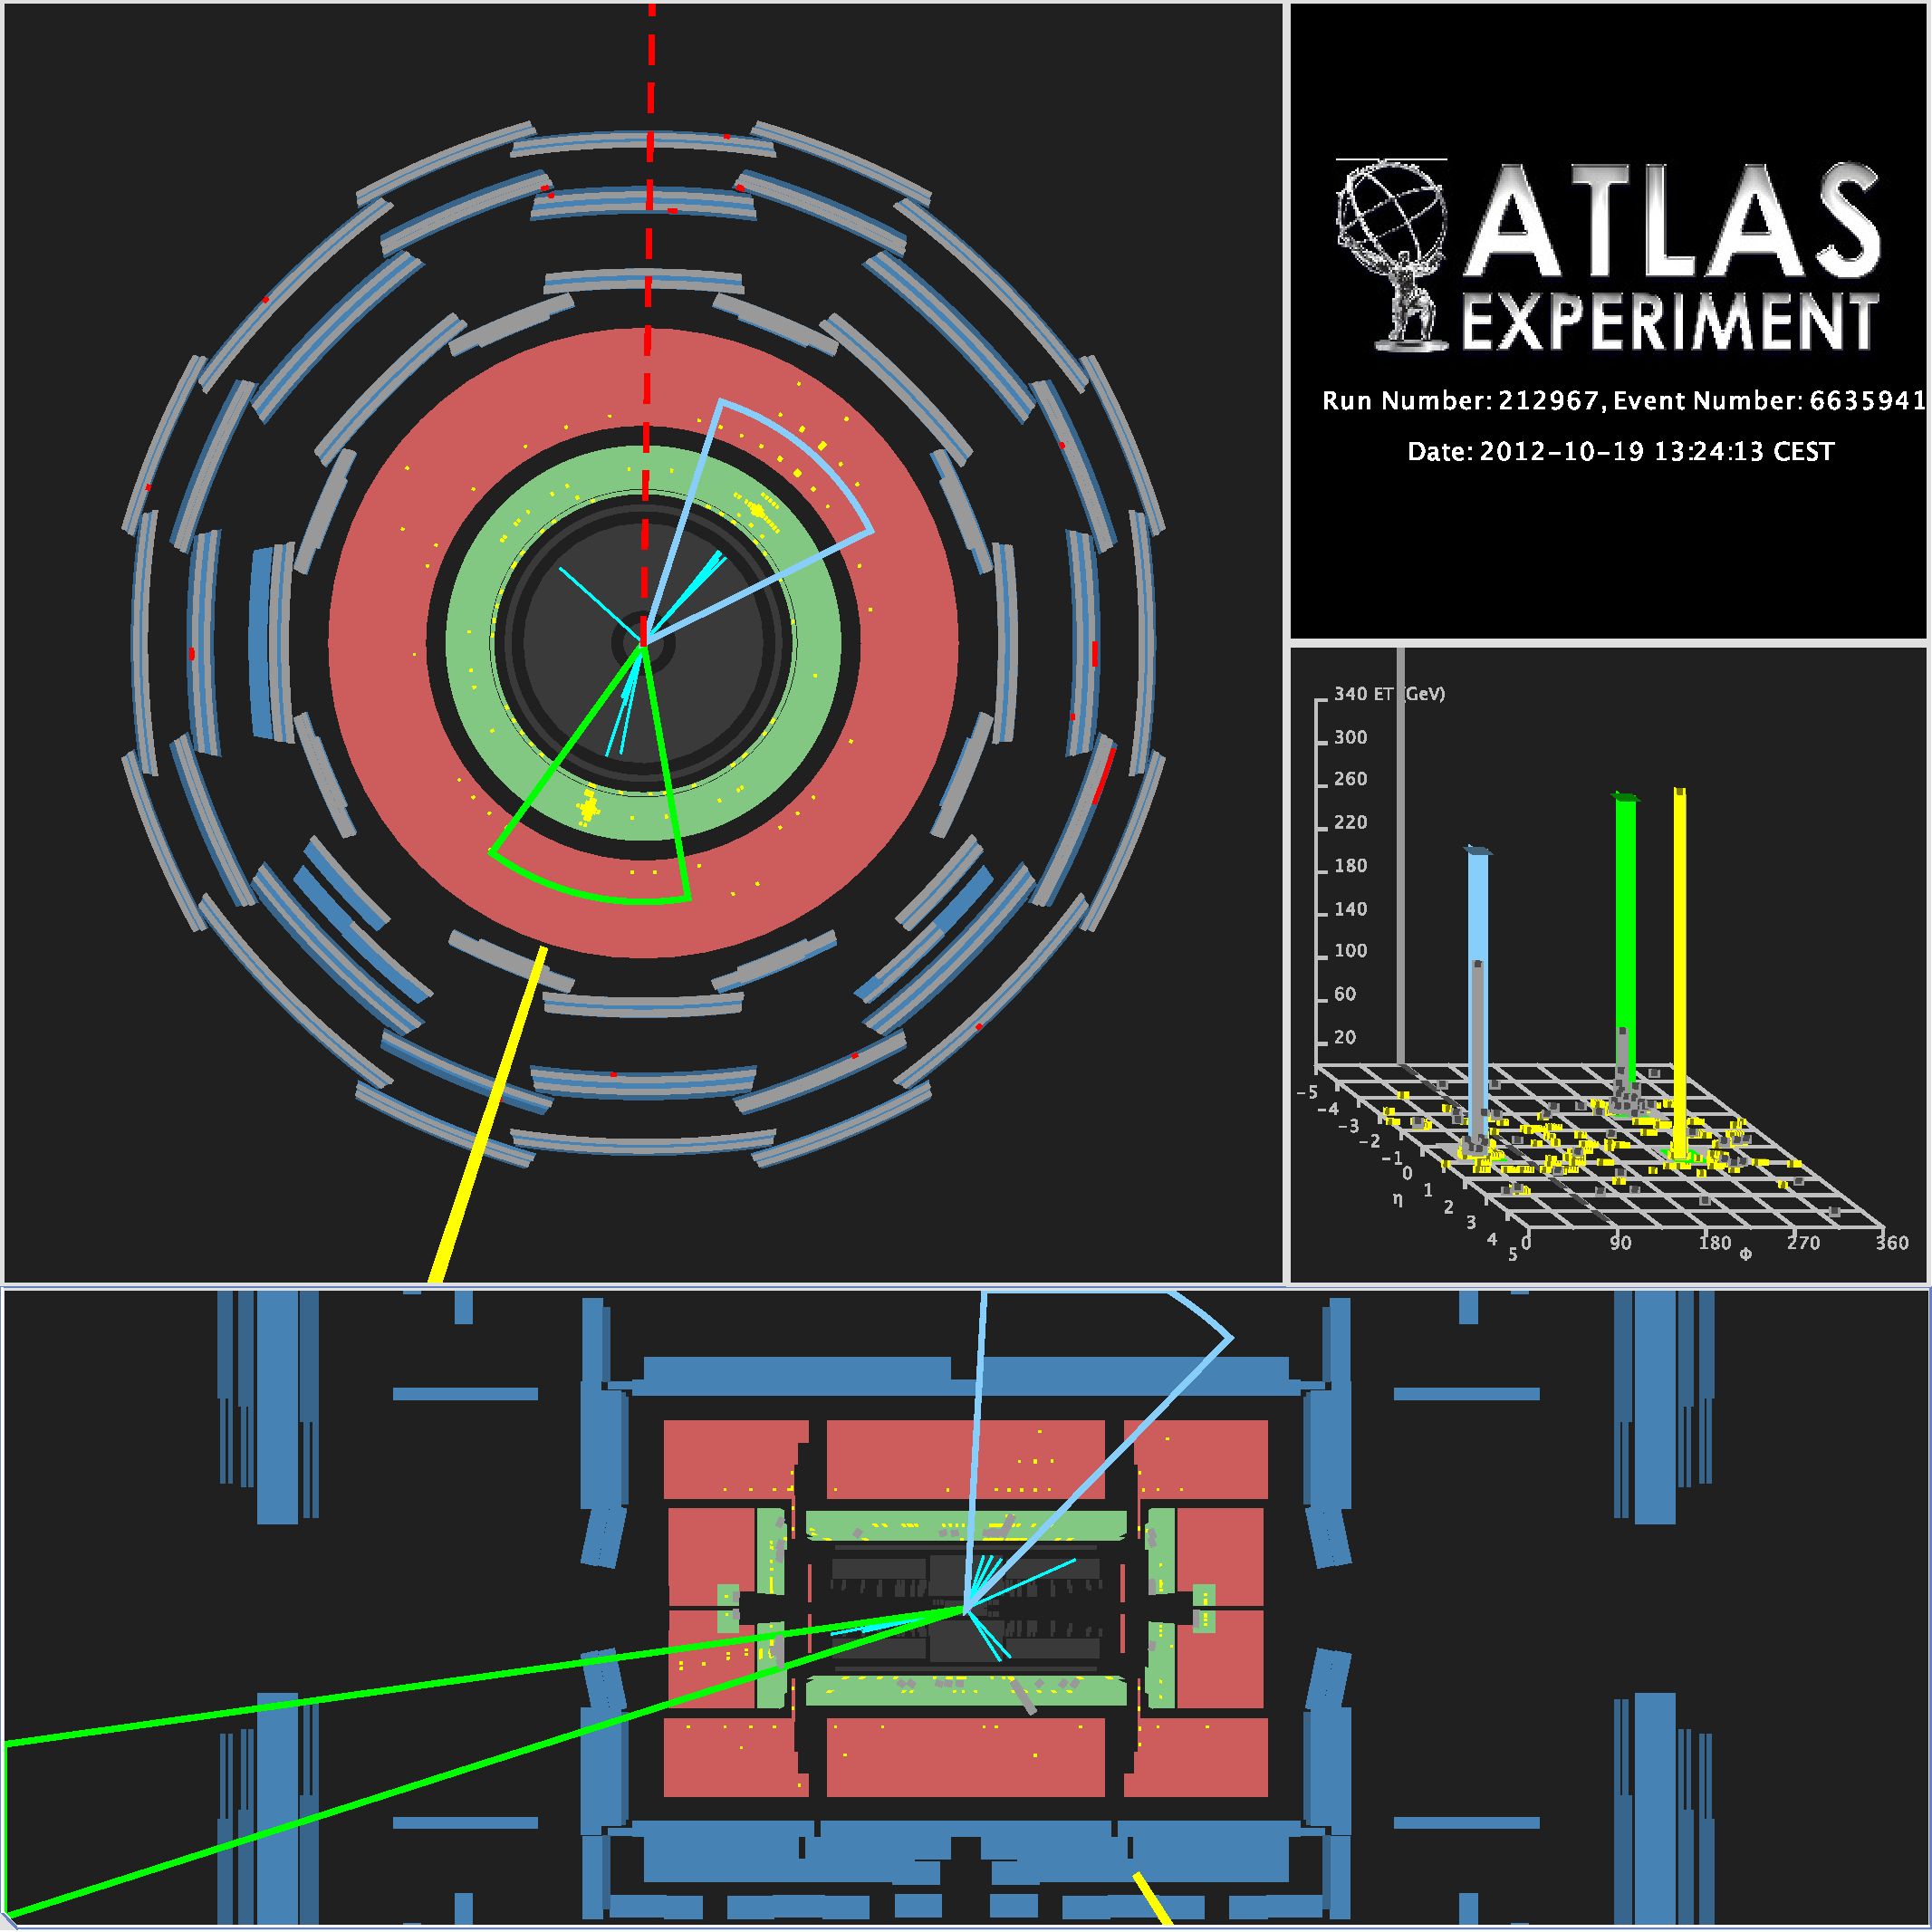
\includegraphics[height=0.45\textheight]{EvtDisplay_212967_66359411}

  \caption{Visualización de los dos eventos que sobreviven la selección de {\SRH}. Ver detalles en el texto.}
  \label{fig:evdisplay_srh}
  \end{center}
\end{figure}


%% \clearpage


%-------------------------
% Model independent limit
%-------------------------
\section{Límites a procesos de nueva física} \label{sec:model_independent}

%% Mas alla de los límites en el modelo de senal de SUSY estudiado en esta Tesis,
%% el analisis que busca nueva fisica puede imponer límites en el número de eventos
%% de nueva fisica por sobre el fondo esperado en cada SR. De esta forma, para cada
%% modelo de senal de interes, cualquiera puede estimar el número de eventos de
%% senal predichos en una SR y chequear si el modelo es excluido o no de acuerdo a
%% los datos observados en el analisis.


Resulta útil proveer el límite superior en el número de eventos de
nueva física impuesto por los resultados obtenidos, mostrados en la sección
anterior. Este límite, provisto para
cada región de señal, hace posible su aplicación a cualquier otro modelo de
nueva física, a partir del cálculo del número de eventos de señal que se espera
en la región en cuestión y verificando que dicho número no exceda el límite
superior obtenido en el presente análisis. Por supuesto que los valores de eficiencia y aceptancia deben ser
tenidos en cuenta.
Para que puedan realizarse este tipo de interpretaciones de otros modelos, todos
los valores y datos relevantes de este analisis son publicados en \textsc{HepData}
para su utilización \cite{hepdata}.\note{Un poco mas de hepdata}

Con el objetivo de obtener los limites independientes del modelo se realiza un
ajuste combinado teniendo en cuenta las regiones de control y cada una de las
regiones de señal. Se supone que la contaminación de señal en las CR es nula,
pero no se realiza ninguna otra suposición acerca del modelo de nueva física. El
número de eventos de señal en la SR se agrega como el parámetro de interés y se
deja libre en el ajuste. Se realiza un muestreo de este parámetro, y el
límite superior en el número de eventos de nueva física se encuentra para el
valor en el cual el {\cls} cae debajo del 5\%. El límite superior en el número
de eventos puede transformarse en el límite superior de la sección eficaz
visible\footnote{La sección eficaz visible se refiere a que tiene en cuenta
  la aceptancia y eficiencia de la selección del análisis, $\sigma_{\text{vis}} = \epsilon\sigma$}
utilizando la luminosidad considerada en el análisis
(20.3 \ifb).

Los resultados se detallan en la \cref{tab:upperlimits} para las dos regiones de
señal. Debido a que el número esperado de eventos de fondo es bajo y no es
posible utilizar la aproximación asintótica que fuera descriptos en la \cref{sec:aprox},
se utilizaron $\sim 3000$
pseudo-experimentos obtenidos con el método Monte Carlo. El límite en el número
de eventos de nueva física resulta en 5.5 y 5.6 para {\SRL} y {\SRH}
respectivamente, lo cual se traduce en un limite en la sección eficaz visible de
0.27 y 0.28 fb.


\begin{table}[!htbp]
  \centering

  \caption{Límite independiente del modelo de señal a 95\% de CL en la
    sección eficaz visible observada ($\langle\epsilon{\rm \sigma}\rangle_{\rm obs}$),
    y el límite en el número de eventos de nueva física observado
    $S_\text{obs}$ para las dos SR.
    La última línea ($p_0$) indica el {\pvalue} de la hipótesis de solo-fondo.}
  \label{tab:upperlimits}

  \begin{tabularx}{\textwidth}{LRR}
  \hline
  {\bf Region de señal}   &            \SRL &              \SRH \\
  \hline
  Eventos observados      &             $2$ &              $2$  \\
  Eventos esperados SM    & $1.27 \pm 0.43$ &  $0.84 \pm 0.38$  \\
  \hline
  $\avg{\epsilon{\sigma}}_\text{obs} \, [\mathrm{fb}]$  & 0.27  & 0.28 \\
  $S_\text{obs}$  & 5.5 & 5.6 \\
  %%$S_\text{exp}$ & ${4.0}^{+1.6}_{-0.1}$ & ${4.1}^{+1.7}_{-0.1}$ \\
  %% {\clb} & 0.86 & 0.83 \\
  $p_0$  & 0.16 &  0.19 \\
  \hline
\end{tabularx}


\end{table}

%% \hll{Poner el plot del scan para este límite}
%% \hll{Límite 1D para EWK?}


%-------------------------
% SUSY Exclusion limit
%-------------------------
\section{Límites de exclusión en el modelo de SUSY considerado}
\label{sec:susy_limits}

Debido a que no se observa un exceso significativo por encima del fondo esperado
del {\SM} en las regiones de señal, se obtuvieron los límites de exclusión en el
modelo de SUSY considerado. Los límites superiores son obtenidos utilizando el
método del {\cls} descripto en la \cref{sec:limits}. Estos límites son
calculados para la sección eficaz nominal del modelo y también con una sección
eficaz de $\pm 1 \sigma$ en la incerteza teórica, siguiendo la recomendación de
ATLAS y el acuerdo de los experimentos del LHC para presentar los resultados.

La \cref{fig:limit_srs} muestra los límites de exclusión esperados y
observados para las dos SR de forma separada. Los límites fueron obtenidos
utilizando $\sim 20000$ pseudo-experimentos. La línea punteada azul muestra el
límite esperado a 95\% CL, con las bandas amarillas indicando la desviación a
1$\sigma$ teniendo en cuenta las incertezas teóricas y experimentales. Los
límites observados están indicados por las líneas en rojo oscuro, donde la línea
sólida representa el límite nominal y las líneas punteadas representan el límite
para las variaciones de la sección eficaz de la señal debido a la incerteza
teórica en la misma.

Por diseño, la {\SRL} es importante en la zona de neutralinos livianos, mientras que
la {\SRH} cubre la región mas comprimida del espacio de fases. En la
\cref{fig:limit_combined}, se muestra el límite combinando ambas
regiones de señal, eligiendo en cada punto la que provee el mejor límite.


\begin{figure}[!htb]
  \centering

  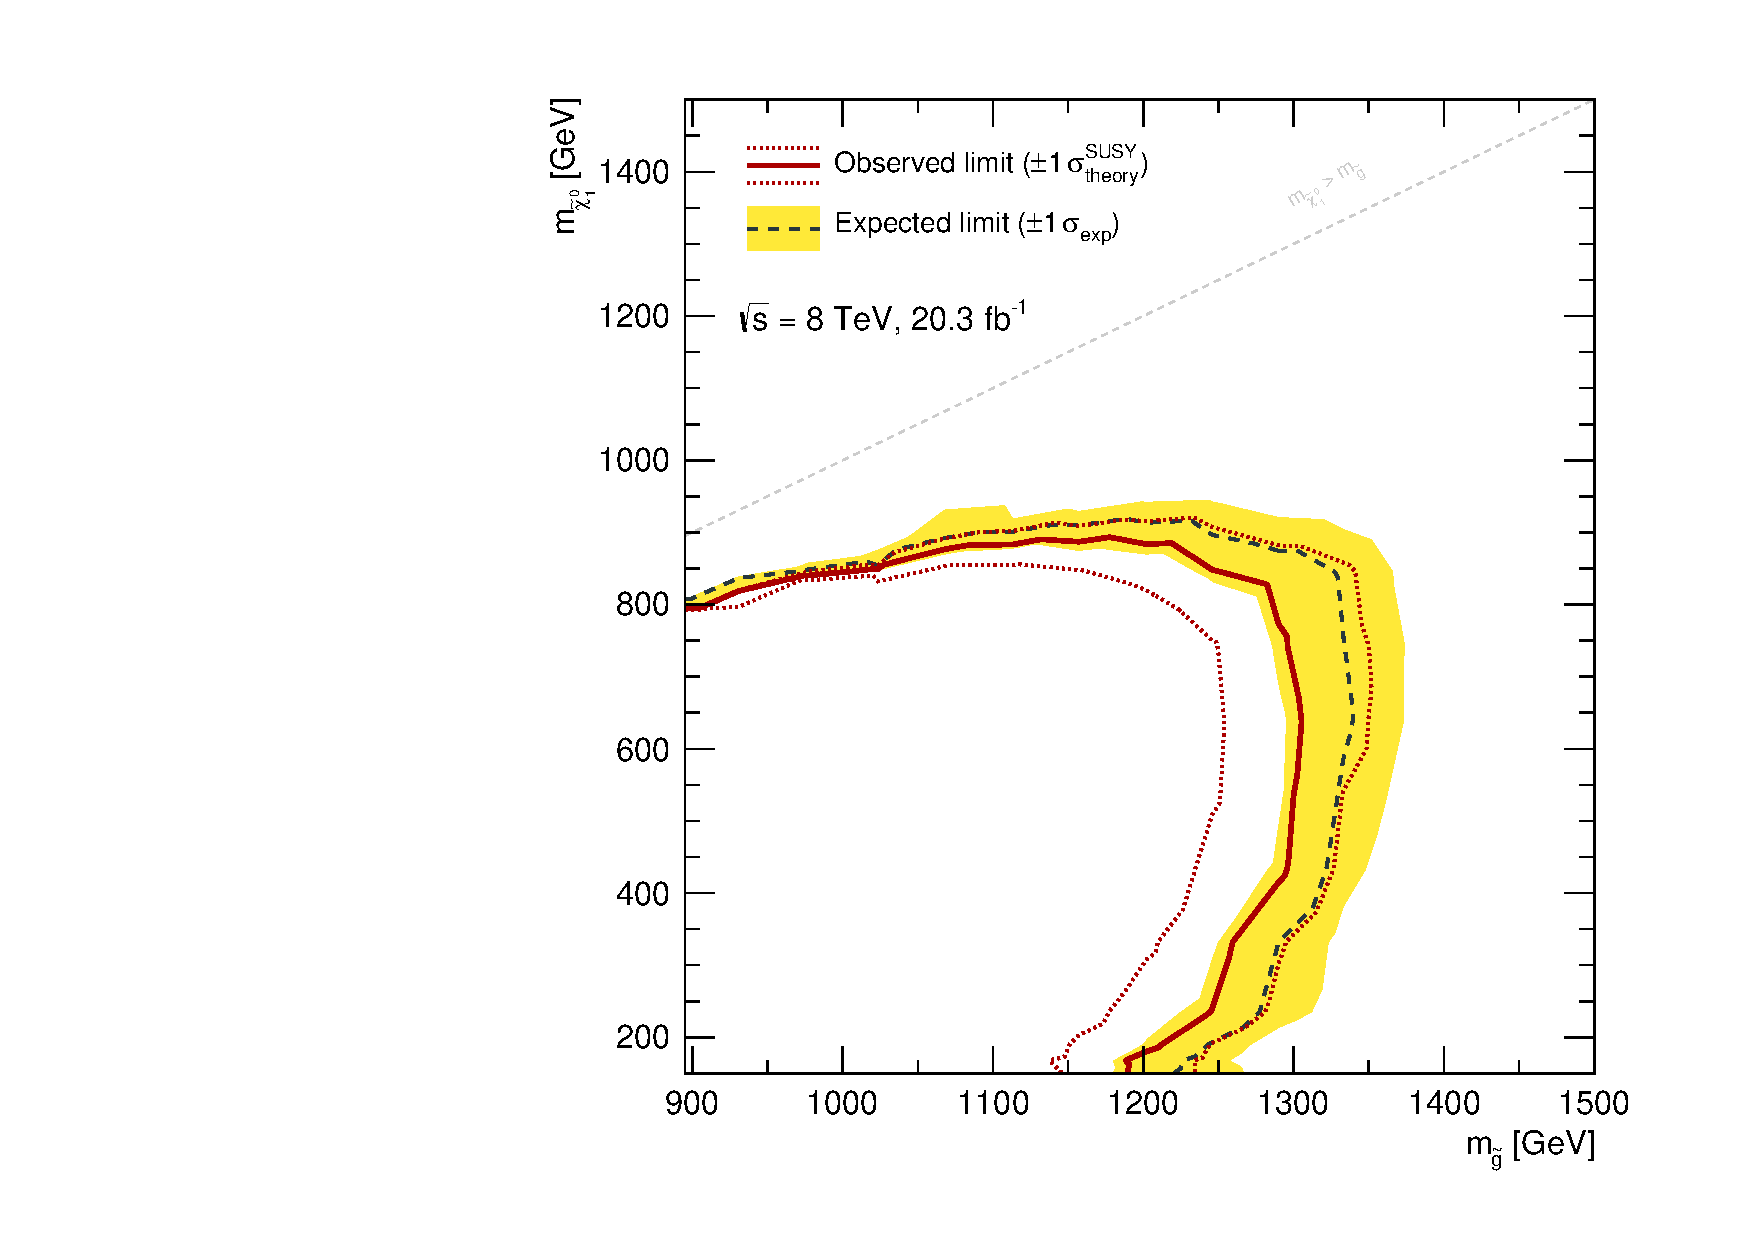
\includegraphics[width=0.49\textwidth]{limitplot_srl}
  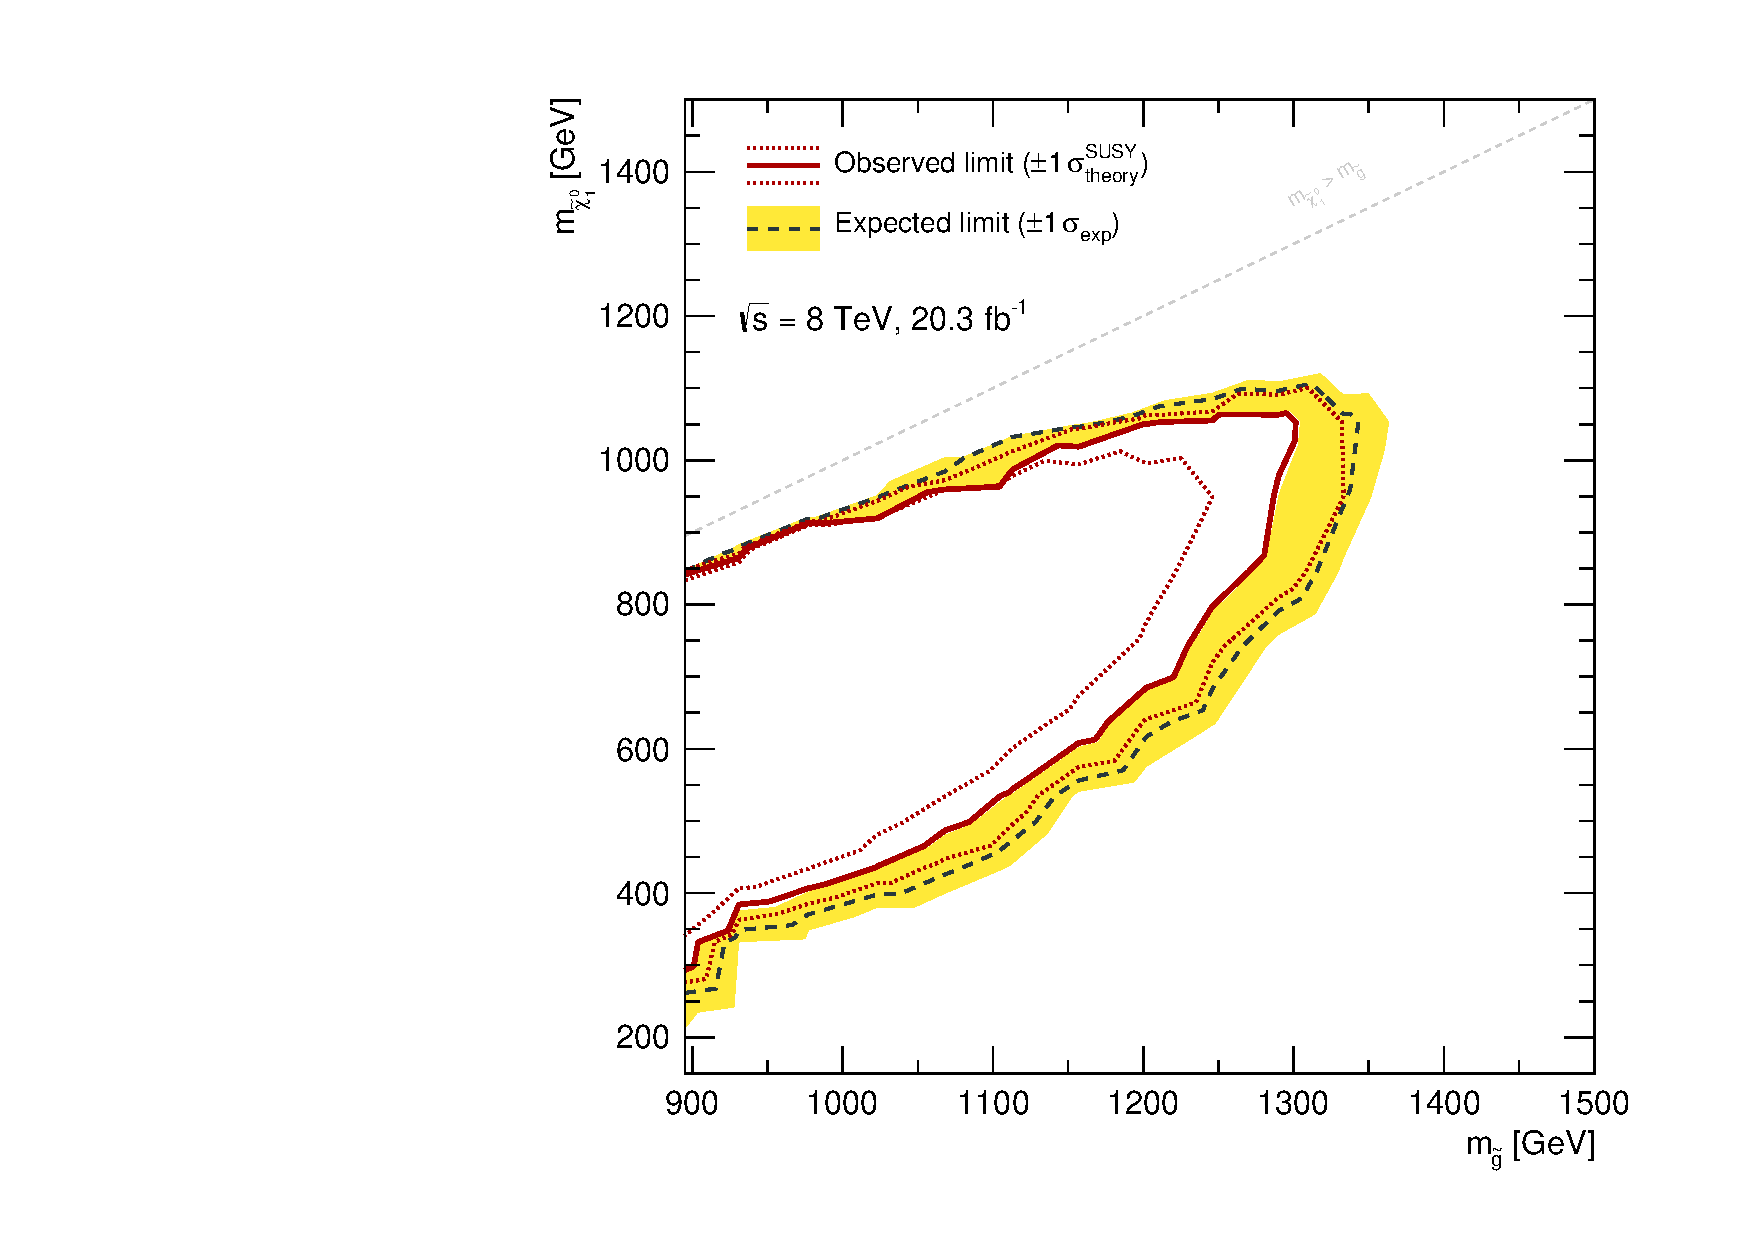
\includegraphics[width=0.49\textwidth]{limitplot_srh}

  \caption{Límites de exclusión a 95\% CL para {\SRL}  (izquierda) y {\SRH} (derecha).}
  \label{fig:limit_srs}
\end{figure}


\begin{figure}[!htb]
  \centering

  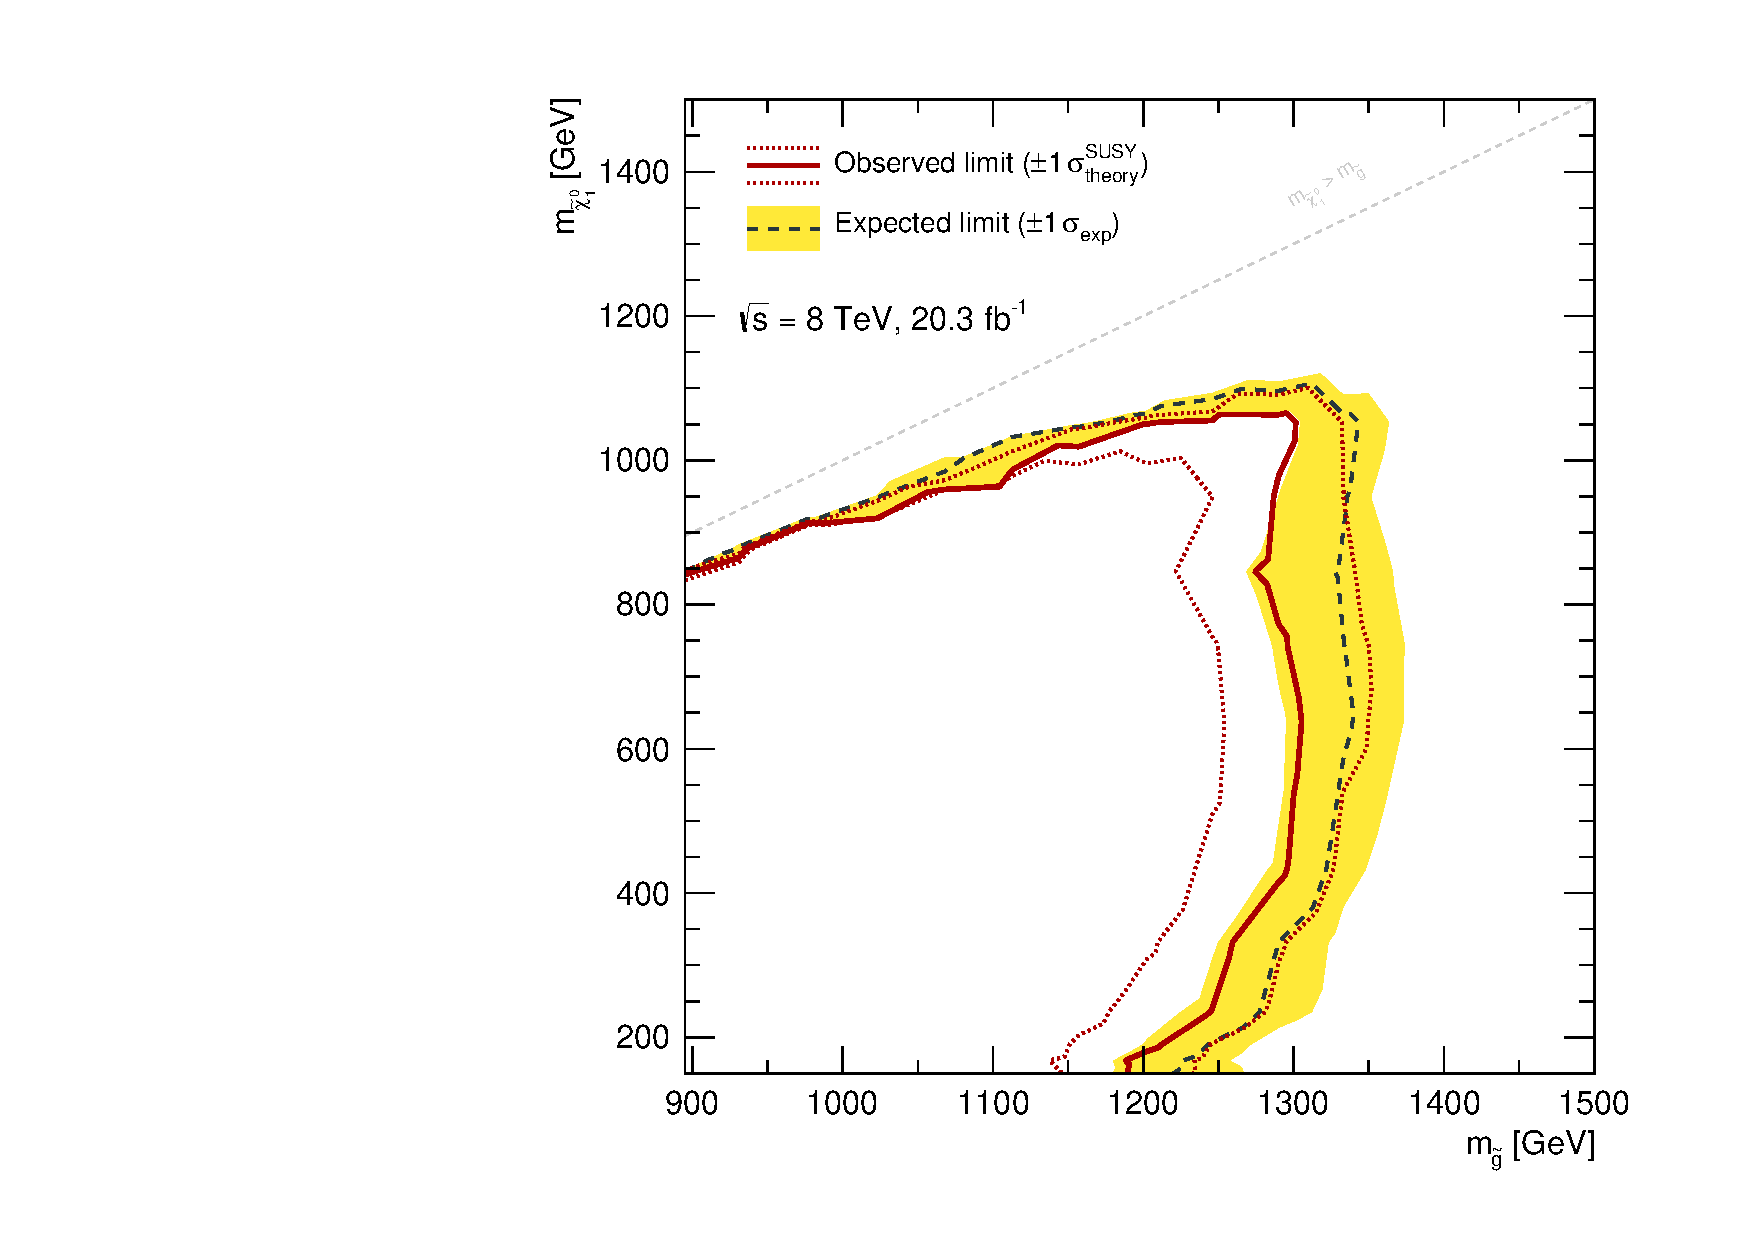
\includegraphics[width=0.8\textwidth]{limitplot_combined}

  \caption{Límites de exclusión para {\SRL} y {\SRH} combinados.
    Los límites son obtenidos usando la región de señal con mejor sensibilidad
    en cada punto.
    La línea punteada azul muestra el límite esperado a 95\% CL, con las bandas amarillas indicando la desviación a
    $1\sigma$ que tiene en cuenta las incertezas teóricas y experimentales. Los
    límites observados están indicados por las lineas en rojo oscuro, donde la línea
    sólida representa el límite nominal y las líneas punteadas representan el límite
    para las variaciones de la sección eficaz de la señal debido a la incerteza
    teórica en la misma.}
   \label{fig:limit_combined}

\end{figure}


Como se desprende de los gráficos de los límites de exclusión, la produccion de
gluino es excluida a 95\% {\cl} para una masa mínima (máxima) de 1190 (1320)
\gev, para $m_{\ninoone}<{840}\gev$. Para masas de gluino menores a $1\tev$, un
neutralino NLSP es excluido entre $150\gev$ y $m_{\gluino}-m_{\ninoone}>50\gev$.

A modo de completitud, en la \cref{fig:susy_summary} se presenta un resumen de los límites obtenidos en
las masas de las partículas supersimétricas buscadas en una selección de los
análisis más sensibles realizados por ATLAS. La Figura incluye el resultado obtenido
por el análisis presentado en esta Tesis, al igual que los análisis
complementarios de búsqueda de modelos GGM \note{Citar aca nuestro paper?}.


\begin{figure}[!htb]
  \centering

  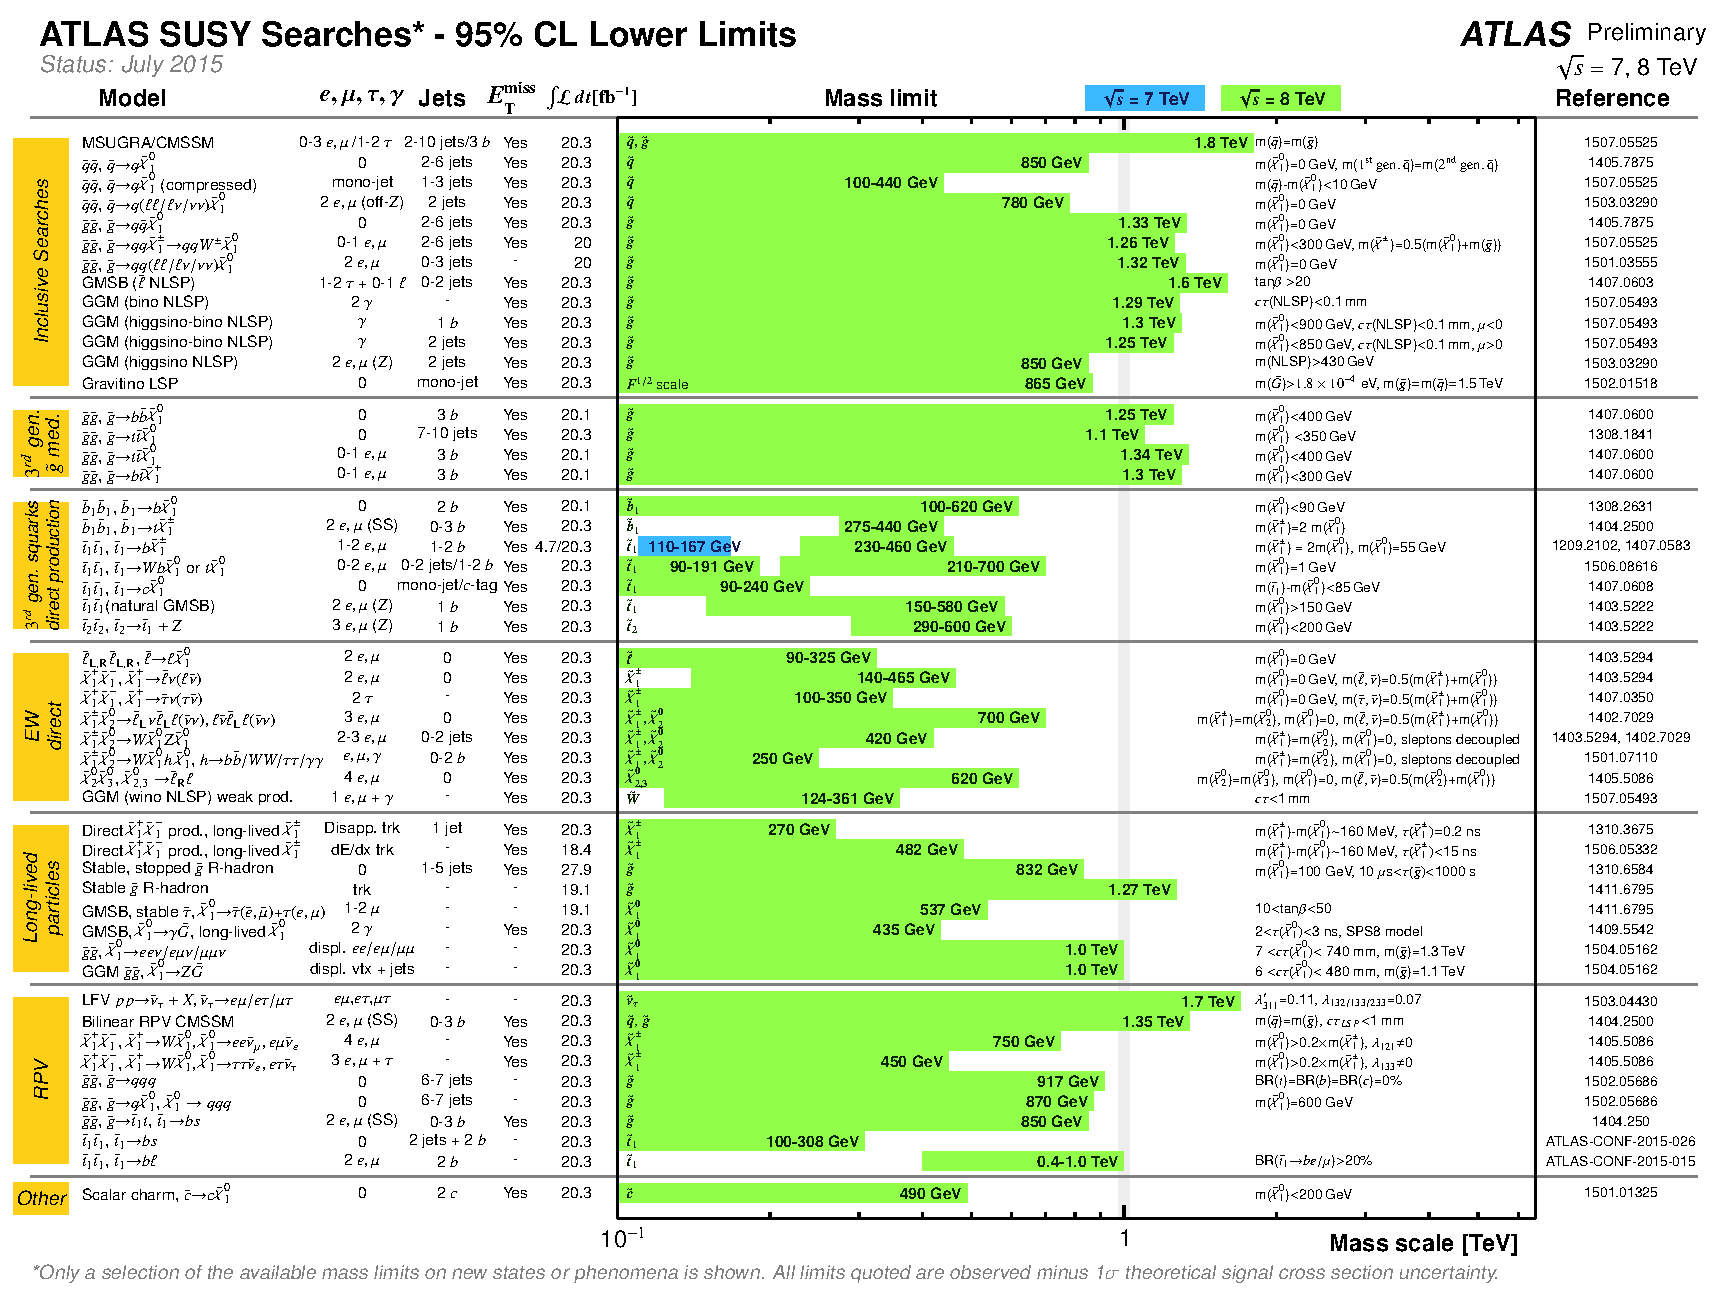
\includegraphics[width=\textwidth]{atlas_susy_run1_summary}

  \caption{Resumen de los límites de exclusión en la masa de las párticulas
    supersimétricas por distintos análisis realizados en ATLAS. Solo una
    selección representativa de los resultados disponibles es
    presentada\cite{susy_summary}, incluyendo los obtenidos en esta Tesis.}
  \label{fig:susy_summary}

\end{figure}


\section{Resultados con 13 \tev}
\label{sec:13tev}

\hl{Agregar}
